\documentclass{article}

\title{Lab 2 - Filters and histogram equalization\\
	\large{Computer Vision}}
\author{Alberto Pasqualetto, 2121718}
\date{24 March 2024}

\usepackage[english]{babel}
% \usepackage{parskip}
\usepackage{float}
\usepackage{graphicx}
\usepackage{caption}
\usepackage{subcaption}
\graphicspath{ {./Images/} }
\usepackage{cleveref}


% \newcommand{\mV}{\,\mathrm{mV}}


\begin{document}
\maketitle


\section*{Task 1}
The first task is pretty straightforward, it asks to convert a provided image into grayscale and then save it. An example at figure \ref{fig:color_to_grayscale}.
\begin{figure}[H]
	\centering
	\begin{subfigure}{0.4\textwidth}
		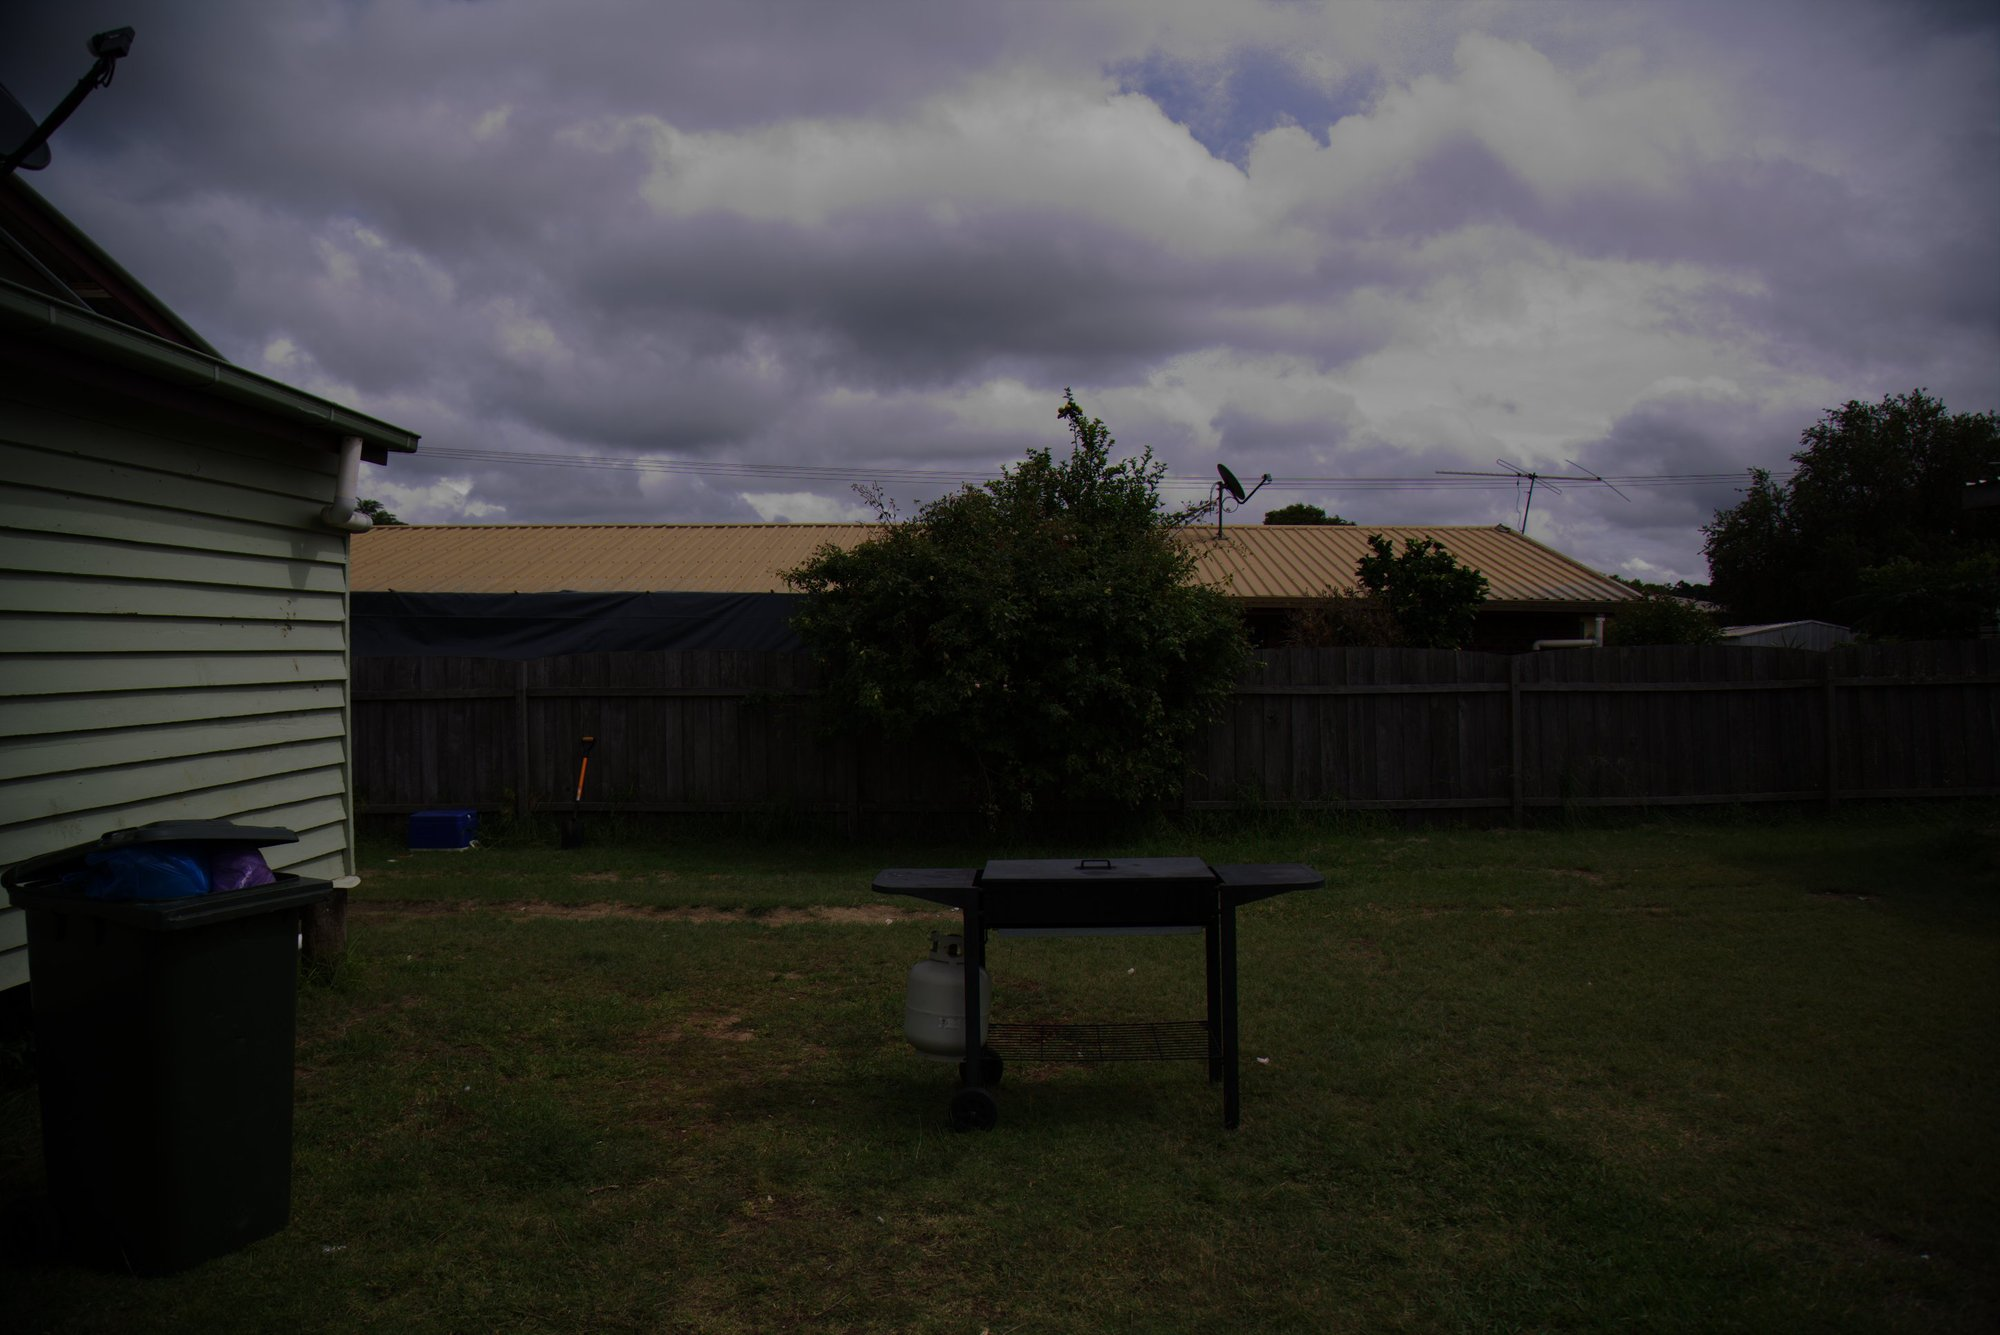
\includegraphics[width=\textwidth]{Garden.jpg}
		\caption{Example of original image}
	\end{subfigure}
	\hfill
	\begin{subfigure}{0.4\textwidth}
		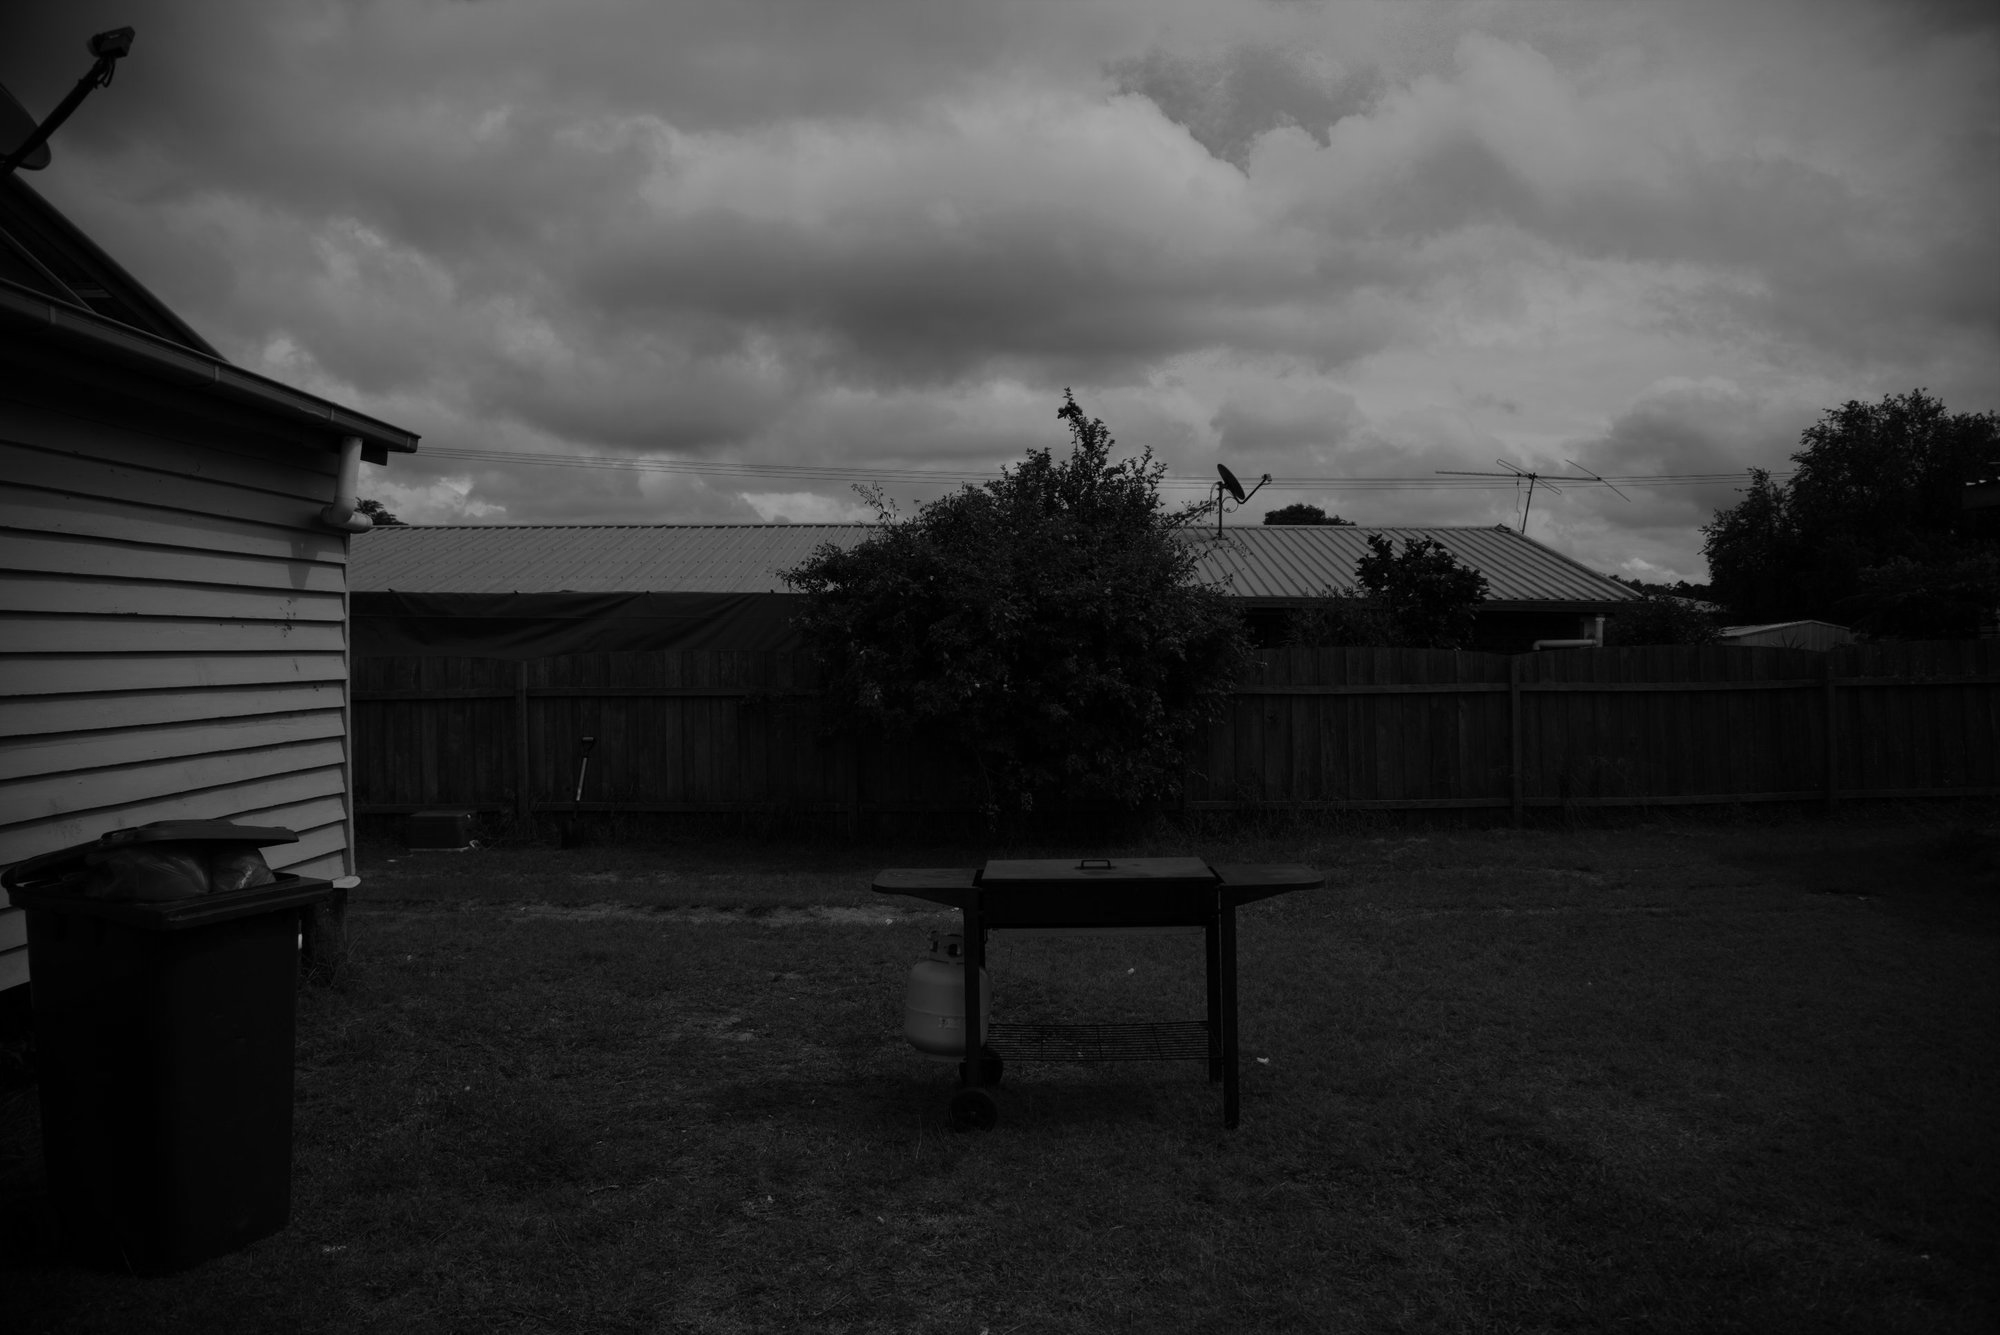
\includegraphics[width=\textwidth]{Generated/Garden_grayscale.png}
		\caption{Grayscale image}
	\end{subfigure}
	\caption{Example of conversion to grayscale}
	\label{fig:color_to_grayscale}
\end{figure}


\section*{Task 2}
Task 2 requires to implement a max and a min filter as functions.
They are implemented taking an image as \texttt{cv::Mat} and a provided kernel size as input.
In order to apply the kernel on every single pixel, a new image with a padding of \texttt{kernelSize/2} is used to compute the result.
The padding is set to the maximum value of the image (255 assuming an \texttt{uchar} type) for the min filter and to the minimum value (0) for the max filter, so that the filter will not be affected by the border.

In "Lena\_corrupted" image, min and max filters behave very badly, as they are not able to recover the original image. If both filters are applied one after the other the results are still bad, but they give a better visualization of the corrupted image. The second filter can also have a bigger kernel. Order of application only changes the final brightness.
The results are shown in figure \ref{fig:min_max_Lena}.
\begin{figure}[H]
	\centering
	\begin{subfigure}{0.4\textwidth}
		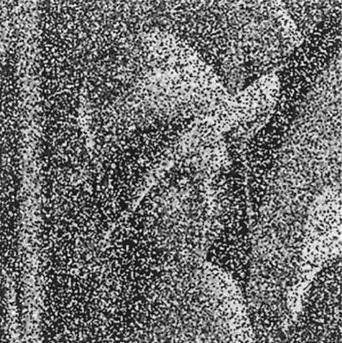
\includegraphics[width=\textwidth]{Lena_corrupted.png}
		\caption{Corrupted image}
	\end{subfigure}
	\hfill
	\begin{subfigure}{0.4\textwidth}
		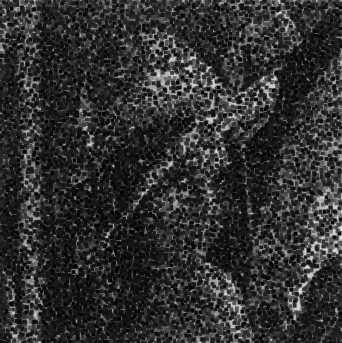
\includegraphics[width=\textwidth]{Generated/Lena_corrupted_min3filter.png}
		\caption{Min filter (kernel 3)}
	\end{subfigure}
	\begin{subfigure}{0.4\textwidth}
		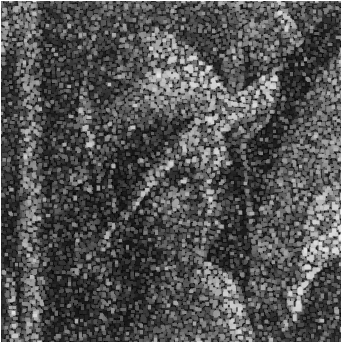
\includegraphics[width=\textwidth]{Generated/Lena_corrupted_min3max3filter.png}
		\caption{Min (kernel 3) then max (kernel 3) filter}
	\end{subfigure}
	\hfill
	\begin{subfigure}{0.4\textwidth}
		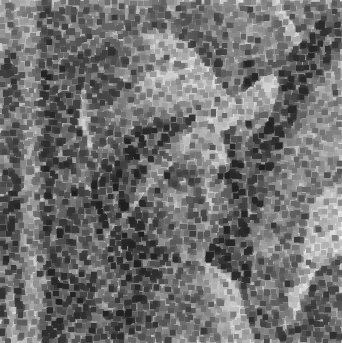
\includegraphics[width=\textwidth]{Generated/Lena_corrupted_max3min5filter.png}
		\caption{Max (kernel 3) then min (kernel 5) filter}
	\end{subfigure}
	\caption{Min and max filter on corrupted Lena}
	\label{fig:min_max_Lena}
\end{figure}

In "Astronaut\_salt\_pepper" image, with salt and pepper noise, applying a single filter, makes the image even worse (kernels greater than 3 are even worse). Applying both filters one after the other the salt (min, then max) or the pepper (max, then min) is almost removed and the other is not affected. If using larger kernels in the second pass (5 is the sweet spot), the image content is more clear since it has less white/black peaks, but it is more blurry and many small squares can be seen.
The results are shown in figure \ref{fig:min_max_Astronaut}.
\begin{figure}[H]
	\centering
	\begin{subfigure}{0.5\textwidth}
		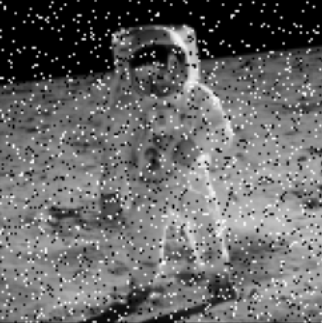
\includegraphics[width=\textwidth]{Astronaut_salt_pepper.png}
		\caption{Corrupted image}
	\end{subfigure}

	\begin{subfigure}{0.4\textwidth}
		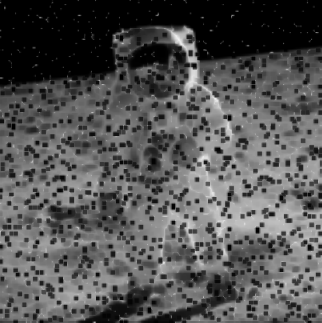
\includegraphics[width=\textwidth]{Generated/Astronaut_salt_pepper_min3filter.png}
		\caption{Min filter (kernel 3)}
	\end{subfigure}
	\hfill
	\begin{subfigure}{0.4\textwidth}
		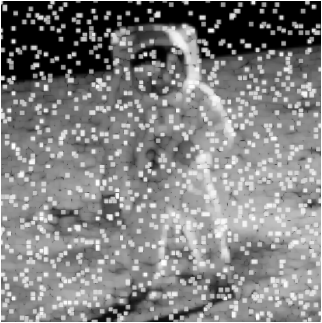
\includegraphics[width=\textwidth]{Generated/Astronaut_salt_pepper_max3filter.png}
		\caption{Max filter (kernel 3)}
	\end{subfigure}

	\begin{subfigure}{0.4\textwidth}
		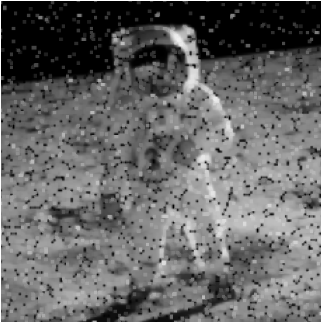
\includegraphics[width=\textwidth]{Generated/Astronaut_salt_pepper_min3max3filter.png}
		\caption{Min (kernel 3) then max (kernel 3) filter}
	\end{subfigure}
	\hfill
	\begin{subfigure}{0.4\textwidth}
		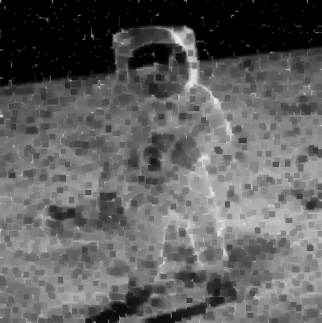
\includegraphics[width=\textwidth]{Generated/Astronaut_salt_pepper_max3min5filter.png}
		\caption{Max (kernel 3) then min (kernel 5) filter}
	\end{subfigure}
	\caption{Min and max filter on corrupted Astronaut}
	\label{fig:min_max_Astronaut}
\end{figure}

In "Garden" image the aim is removing the electric cables. Applying a max filter with kernel 3 removes all but one cables without any artifact, with kernel 5 it removes all cables introducing some artifacts especially on the tree; if a min filter with kernel 3 is applied after the max with kernel 5, the results are even better, reducing artifacts on the tree.
If min filter is applied first, electric cables are not removed because cables are black. therefore they are the minimum value when kernel is applied; increasing kernel size introduces too much artifacts.
The results are shown in figure \ref{fig:min_max_Garden}.
\begin{figure}[H]
	\centering
	\begin{subfigure}{0.45\textwidth}
		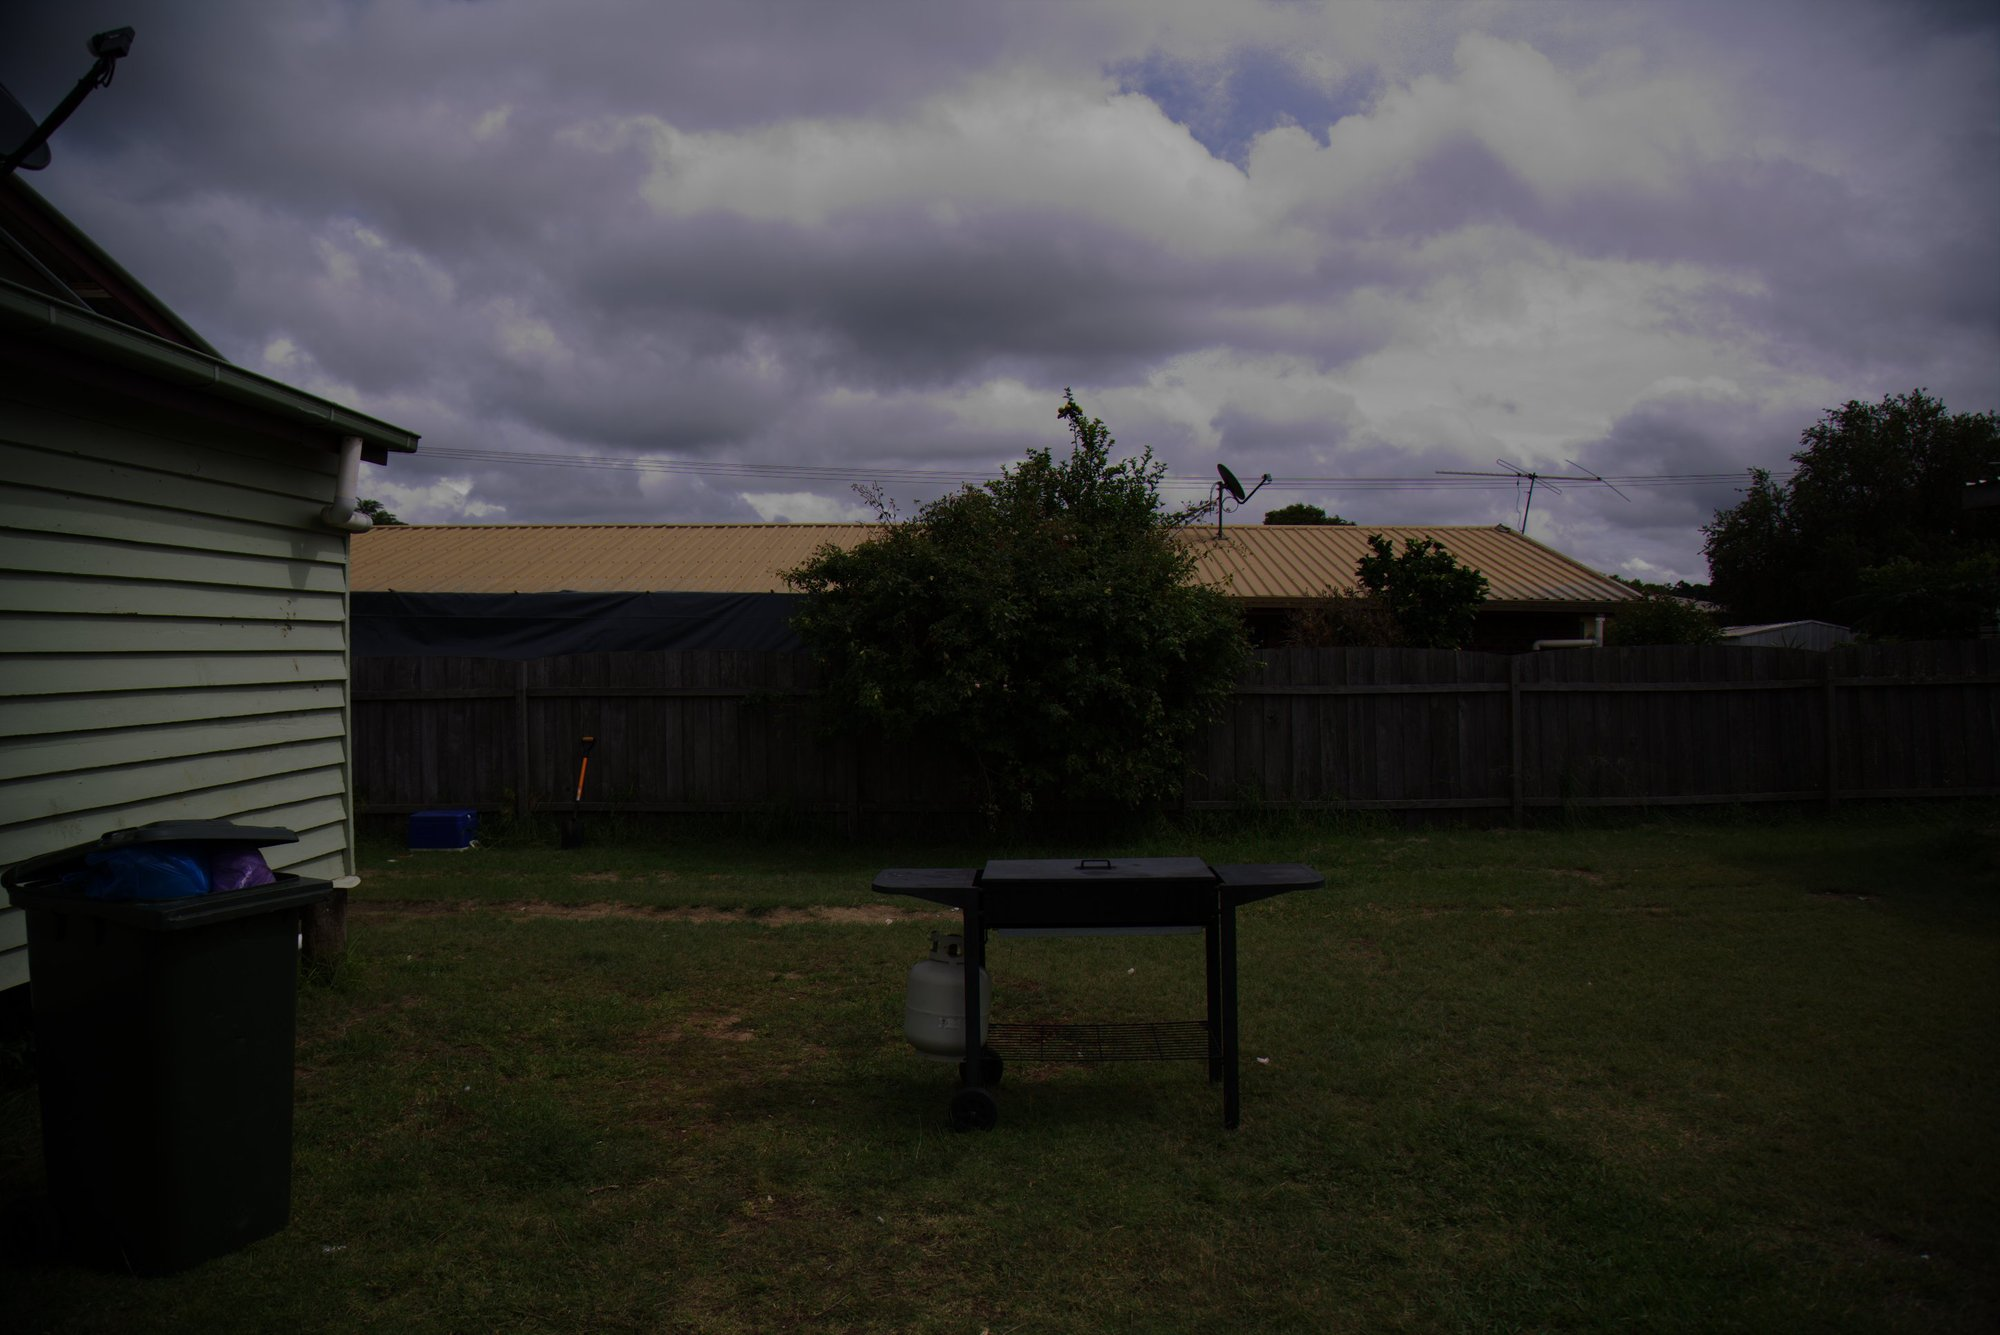
\includegraphics[trim={20cm 25cm 25cm 10cm},clip,width=\textwidth]{Garden.jpg}
		\caption{Original image (cropped)}
	\end{subfigure}

	\begin{subfigure}{0.45\textwidth}
		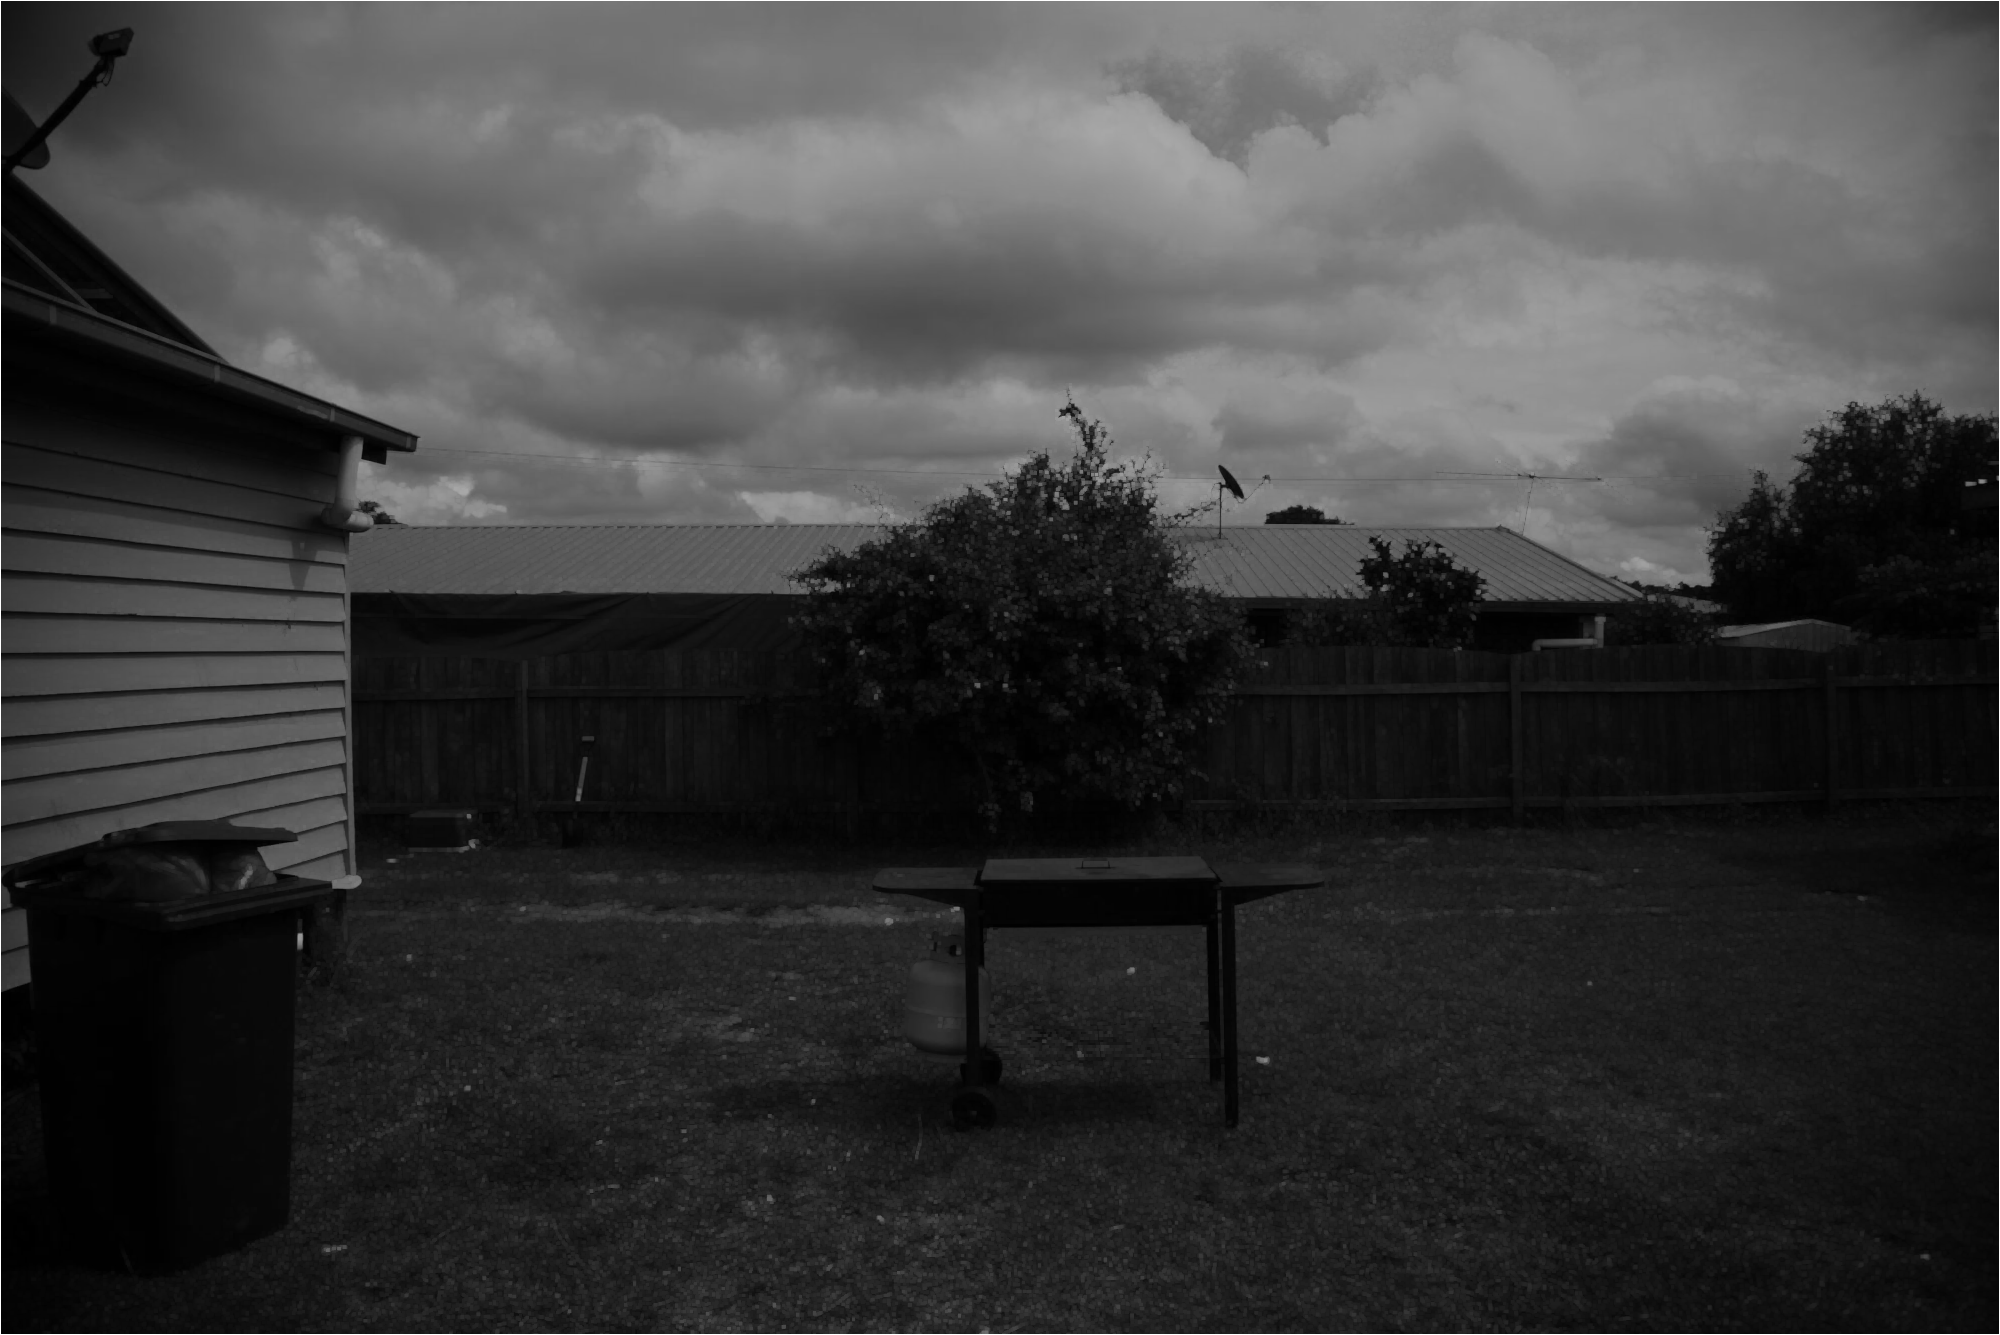
\includegraphics[trim={20cm 25cm 25cm 10cm},clip,width=\textwidth]{Generated/Garden_max3filter.png}
		\caption{Max filter (kernel 3) (cropped)}
	\end{subfigure}
	\hfill
	\begin{subfigure}{0.45\textwidth}
		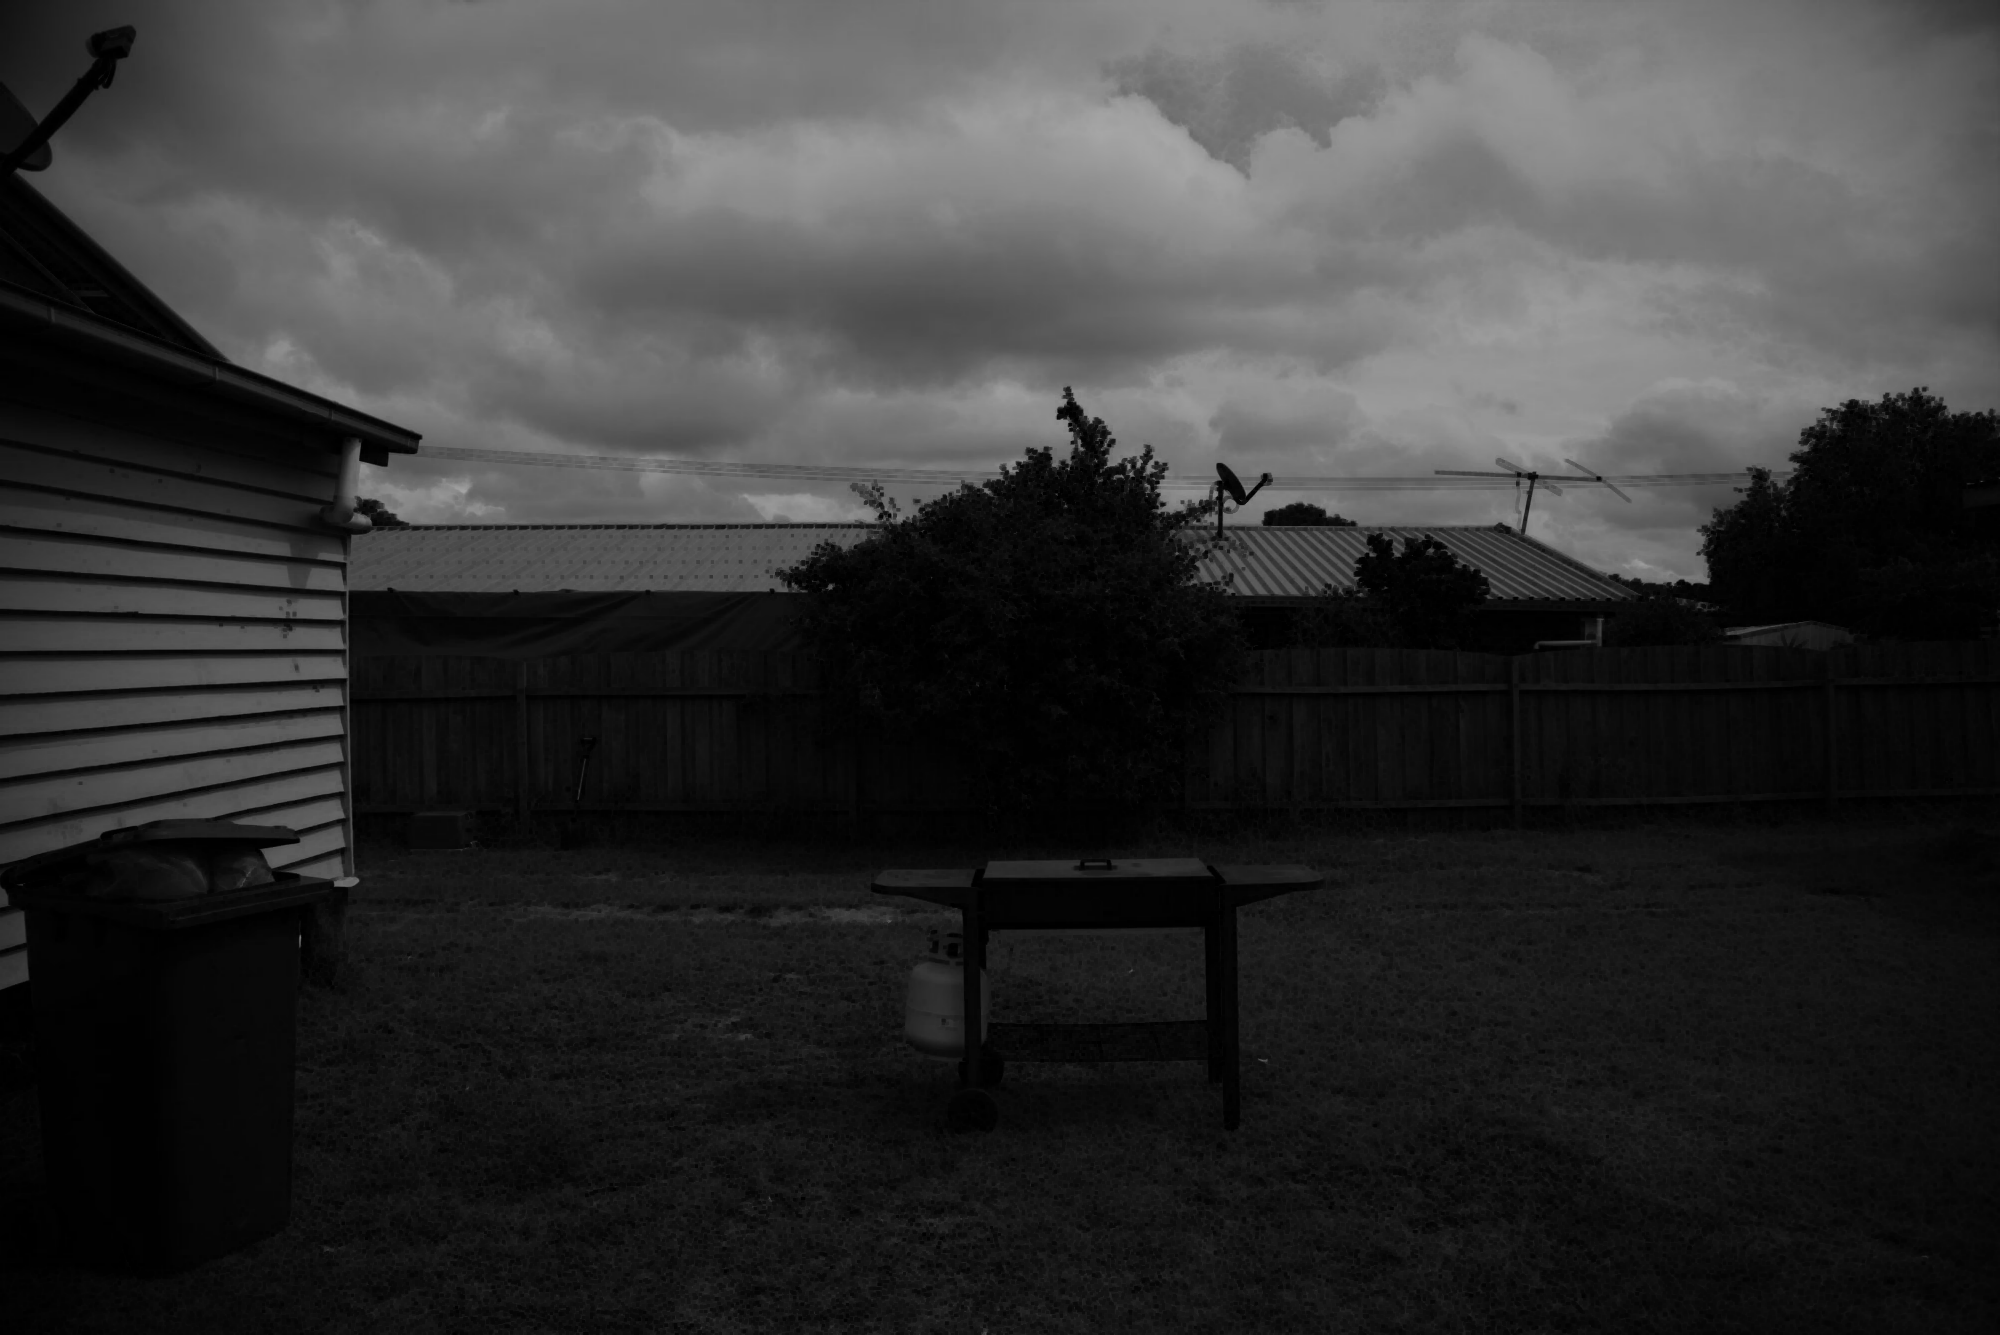
\includegraphics[trim={20cm 25cm 25cm 10cm},clip,width=\textwidth]{Generated/Garden_min3filter.png}
		\caption{Min filter (kernel 3) (cropped)}
	\end{subfigure}
	\begin{subfigure}{0.45\textwidth}
		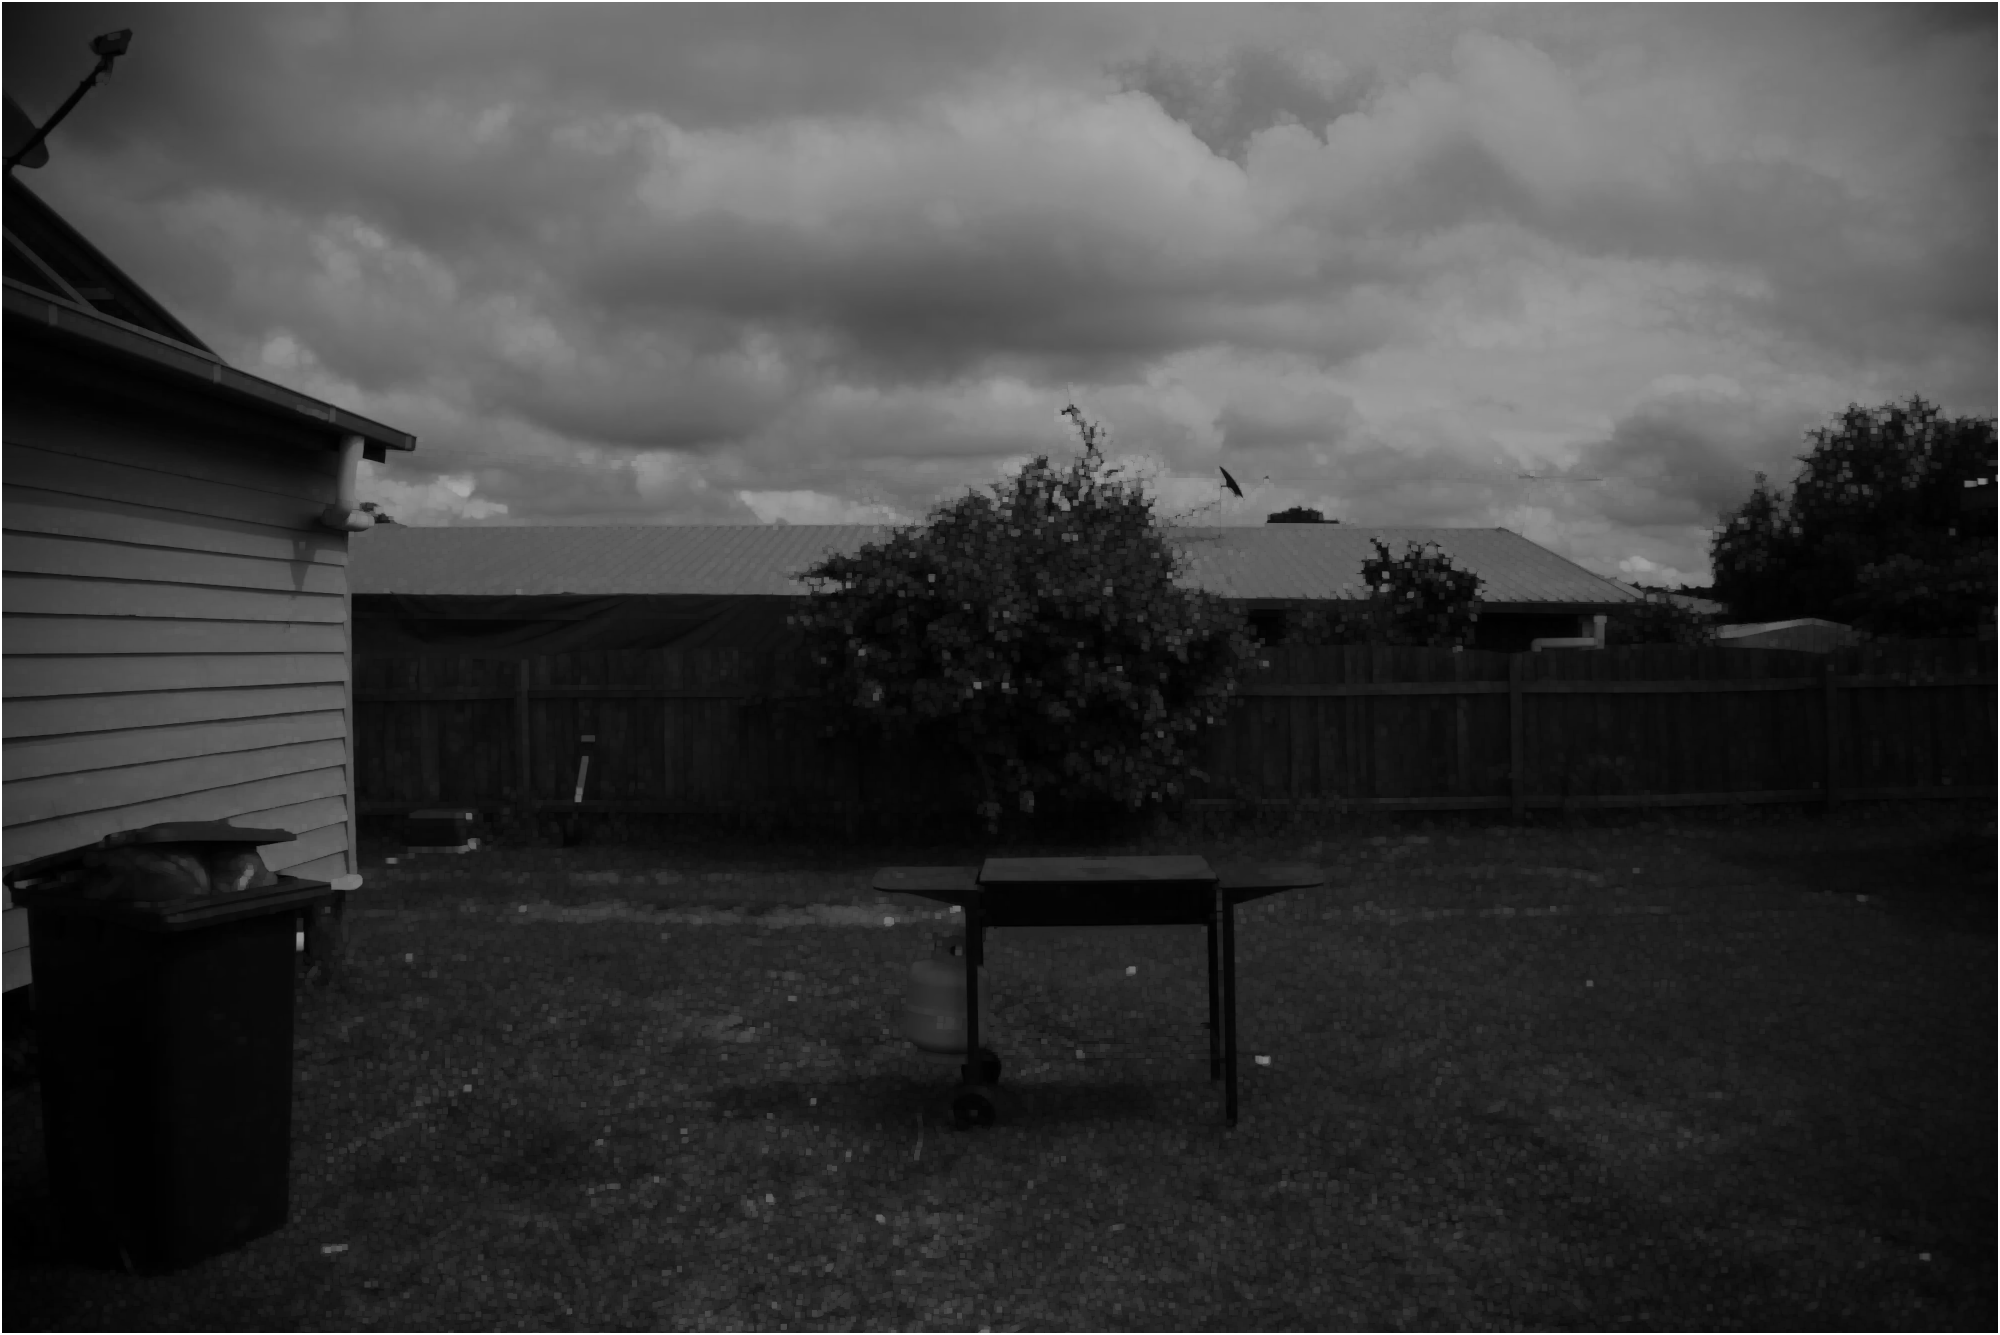
\includegraphics[trim={20cm 25cm 25cm 10cm},clip,width=\textwidth]{Generated/Garden_max5filter.png}
		\caption{Max filter (kernel 5) (cropped)}
	\end{subfigure}

	\begin{subfigure}{0.45\textwidth}
		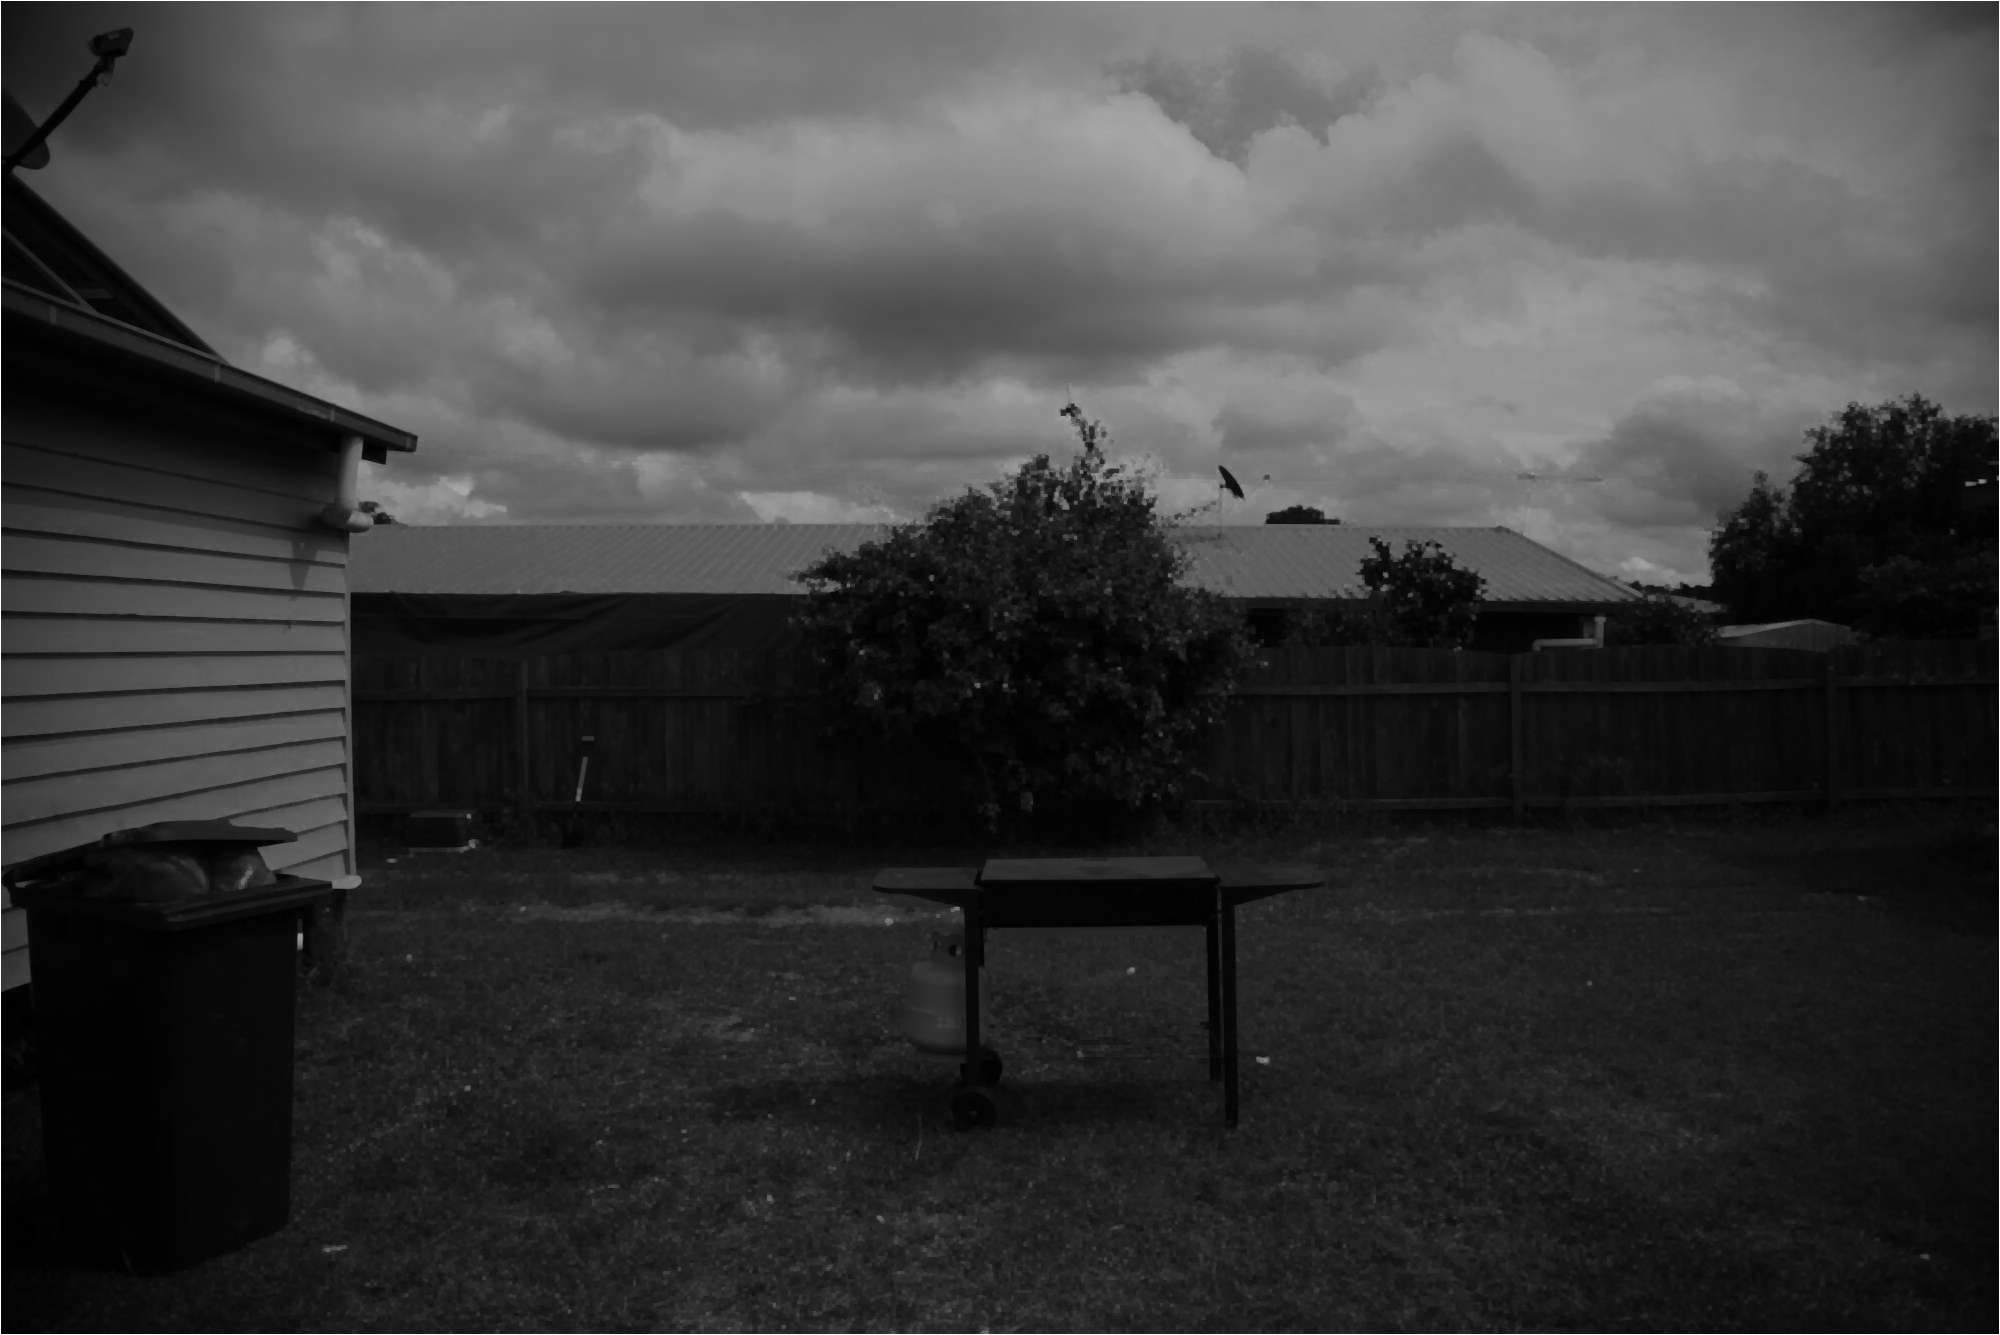
\includegraphics[trim={20cm 25cm 25cm 10cm},clip,width=\textwidth]{Generated/Garden_max5min3filter.png}
		\caption{Max (kernel 5) then min (kernel 3) filter (cropped)}
	\end{subfigure}
	\caption{Min and max filter on Garden}
	\label{fig:min_max_Garden}
\end{figure}


\section*{Task 3}
Median filter is implemented as a function that takes an image as \texttt{cv::Mat} and a kernel size as input, for each kernel to be applied, it sorts the values pushing them to a \texttt{std::vector} and takes the median one.

Median filter performs well in removing noise: in "Lena\_corrupted" kernel 3 gives a better representation than min and max filters (See figure \ref{fig:median3_Lena}) and kernel 5 trades noise with sharpness (See figure \ref{fig:median5_Lena}); in "Astronaut\_salt\_pepper" kernel 3 works, but it works similar to two pass min-max filter with kernel 3 (See figure \ref{fig:median3_Astronaut}).

Median filter does not help at removing electric cables in "Garden" with any kernel (See figure \ref{fig:median3_Garden}).
\begin{figure}[H]
	\centering
	\begin{subfigure}{0.4\textwidth}
		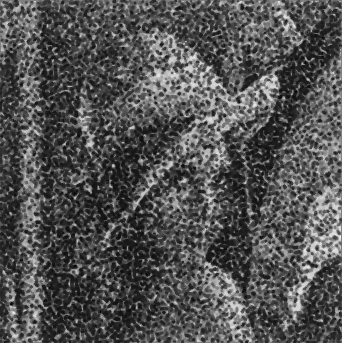
\includegraphics[width=\textwidth]{Generated/Lena_corrupted_median3filter.png}
		\caption{Median filter (kernel 3) on corrupted Lena}
		\label{fig:median3_Lena}
	\end{subfigure}
	\hfill
	\begin{subfigure}{0.4\textwidth}
		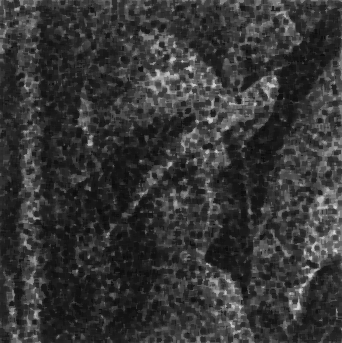
\includegraphics[width=\textwidth]{Generated/Lena_corrupted_median5filter.png}
		\caption{Median filter (kernel 5) on corrupted Lena}
		\label{fig:median5_Lena}
	\end{subfigure}

	\begin{subfigure}{0.4\textwidth}
		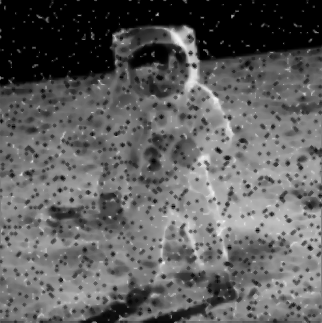
\includegraphics[width=\textwidth]{Generated/Astronaut_salt_pepper_median3filter.png}
		\caption{Median filter (kernel 5) on corrupted Astronaut}
		\label{fig:median3_Astronaut}
	\end{subfigure}

	\begin{subfigure}{0.4\textwidth}
		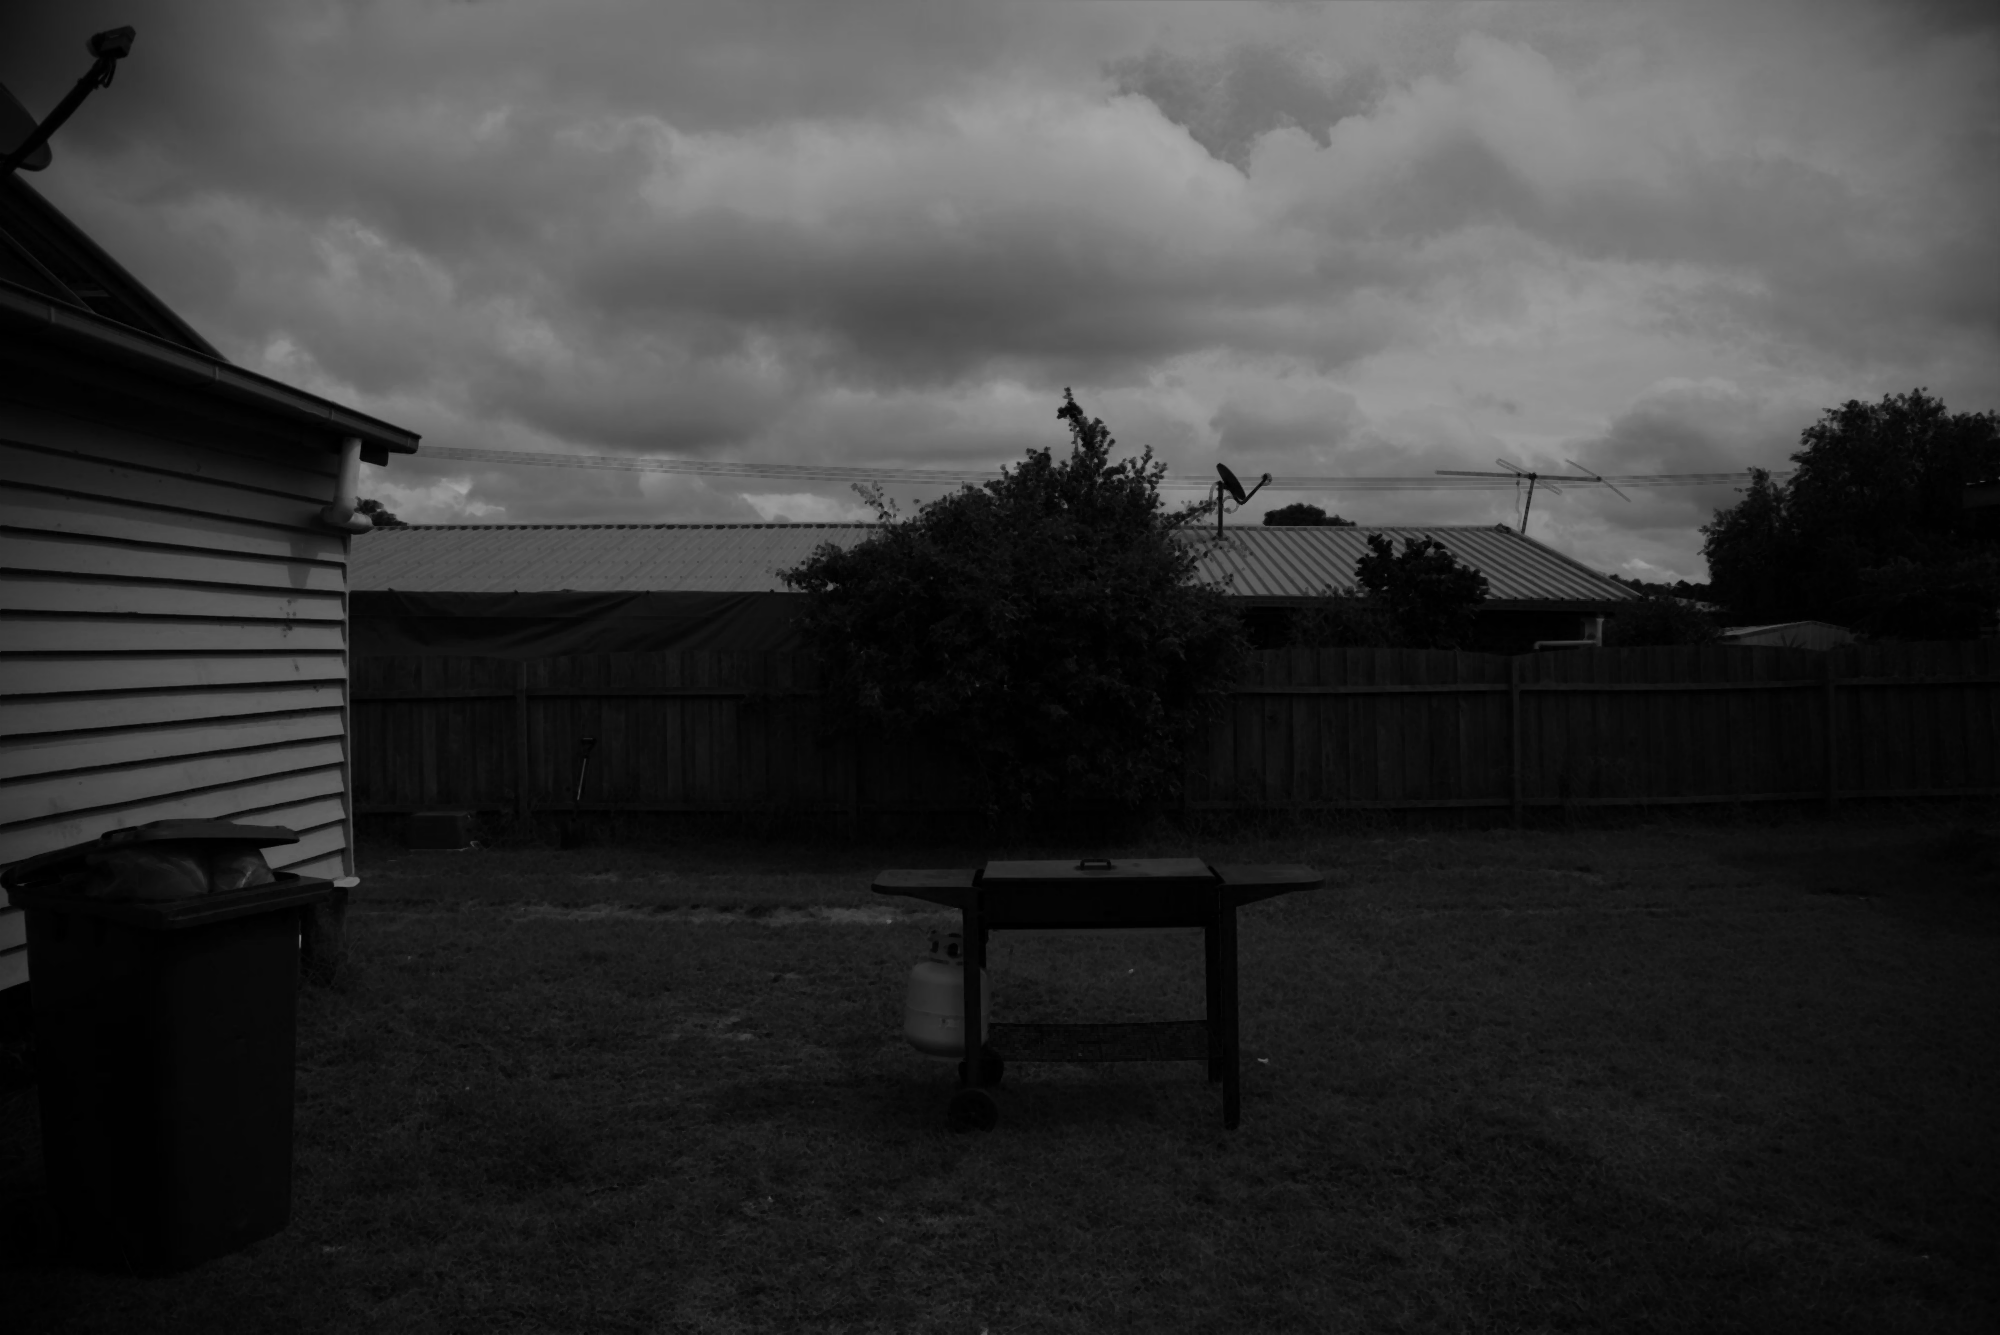
\includegraphics[trim={20cm 25cm 25cm 10cm},clip,width=\textwidth]{Generated/Garden_median3filter.png}
		\caption{Median filter (kernel 3) on Garden (cropped)}
		\label{fig:median3_Garden}
	\end{subfigure}
	\label{Median filter}
\end{figure}


\section*{Task 4}
Gaussian filter is applied using \texttt{cv::GaussianBlur}.

It trades noise with blur increasing kernel size (See figures \labelcref{fig:gaussian3_Lena,fig:gaussian21_Lena,fig:gaussian41_Lena,fig:gaussian3_Astronaut,fig:gaussian21_Astronaut,fig:gaussian41_Astronaut}).
It does not remove electric cables in "Garden" except for high kernels where everything is very blurred. (See figures \labelcref{fig:gaussian3_Garden,fig:gaussian21_Garden,fig:gaussian41_Garden})
\begin{figure}[H]
	\centering
	\begin{subfigure}{0.3\textwidth}
		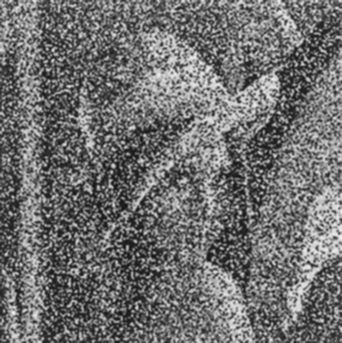
\includegraphics[width=\textwidth]{Generated/Lena_corrupted_gaussian3filter.png}
		\caption{Gaussian filter (kernel 3) on corrupted Lena}
		\label{fig:gaussian3_Lena}
	\end{subfigure}
	\hfill
	\begin{subfigure}{0.3\textwidth}
		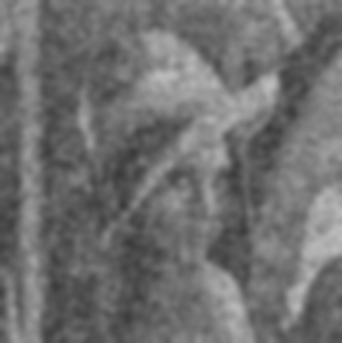
\includegraphics[width=\textwidth]{Generated/Lena_corrupted_gaussian21filter.png}
		\caption{Gaussian filter (kernel 21) on corrupted Lena}
		\label{fig:gaussian21_Lena}
	\end{subfigure}
	\hfill
	\begin{subfigure}{0.3\textwidth}
		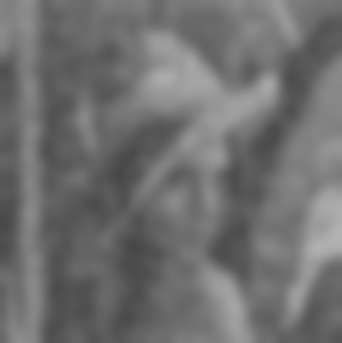
\includegraphics[width=\textwidth]{Generated/Lena_corrupted_gaussian41filter.png}
		\caption{Gaussian filter (kernel 41) on corrupted Lena}
		\label{fig:gaussian41_Lena}
	\end{subfigure}

	\begin{subfigure}{0.3\textwidth}
		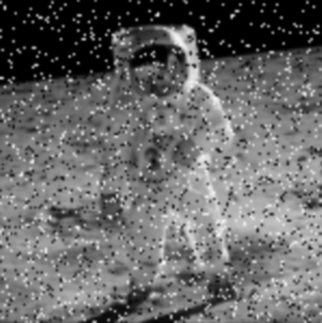
\includegraphics[width=\textwidth]{Generated/Astronaut_salt_pepper_gaussian3filter.png}
		\caption{Gaussian filter (kernel 3) on corrupted Astronaut}
		\label{fig:gaussian3_Astronaut}
	\end{subfigure}
	\hfill
	\begin{subfigure}{0.3\textwidth}
		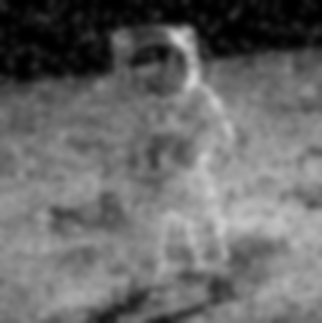
\includegraphics[width=\textwidth]{Generated/Astronaut_salt_pepper_gaussian21filter.png}
		\caption{Gaussian filter (kernel 21) on corrupted Astronaut}
		\label{fig:gaussian21_Astronaut}
	\end{subfigure}
	\hfill
	\begin{subfigure}{0.3\textwidth}
		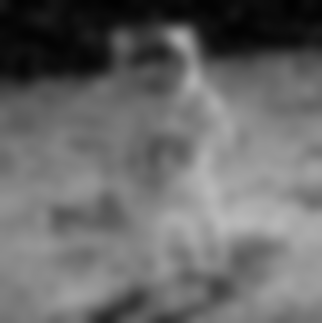
\includegraphics[width=\textwidth]{Generated/Astronaut_salt_pepper_gaussian41filter.png}
		\caption{Gaussian filter (kernel 41) on corrupted Astronaut}
		\label{fig:gaussian41_Astronaut}
	\end{subfigure}

	\begin{subfigure}{0.3\textwidth}
		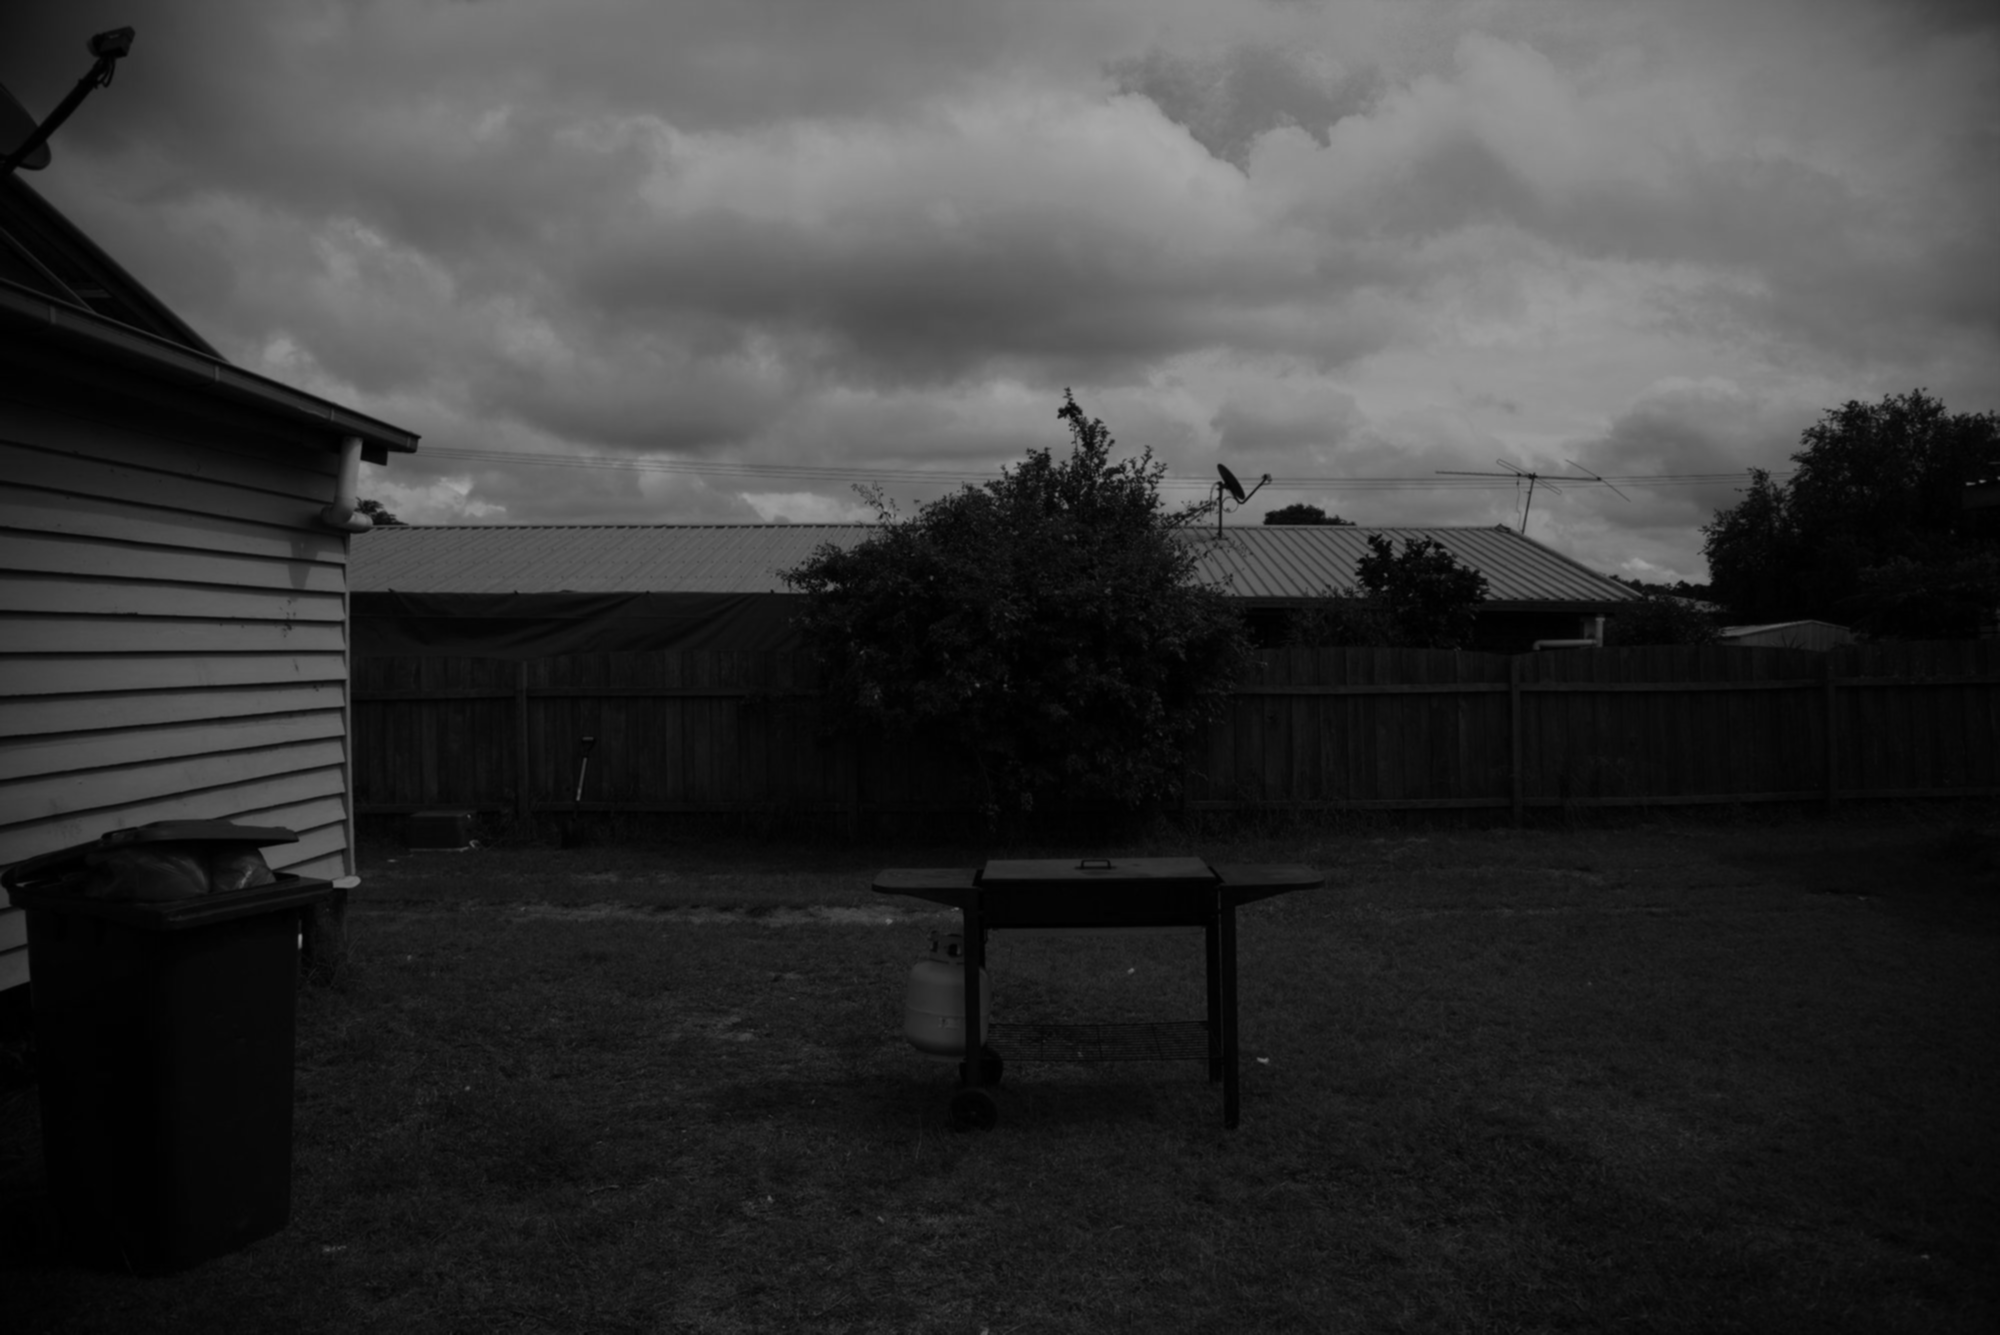
\includegraphics[trim={20cm 25cm 25cm 10cm},clip,width=\textwidth]{Generated/Garden_gaussian3filter.png}
		\caption{Gaussian filter (kernel 3) on Garden (cropped)}
		\label{fig:gaussian3_Garden}
	\end{subfigure}
	\hfill
	\begin{subfigure}{0.3\textwidth}
		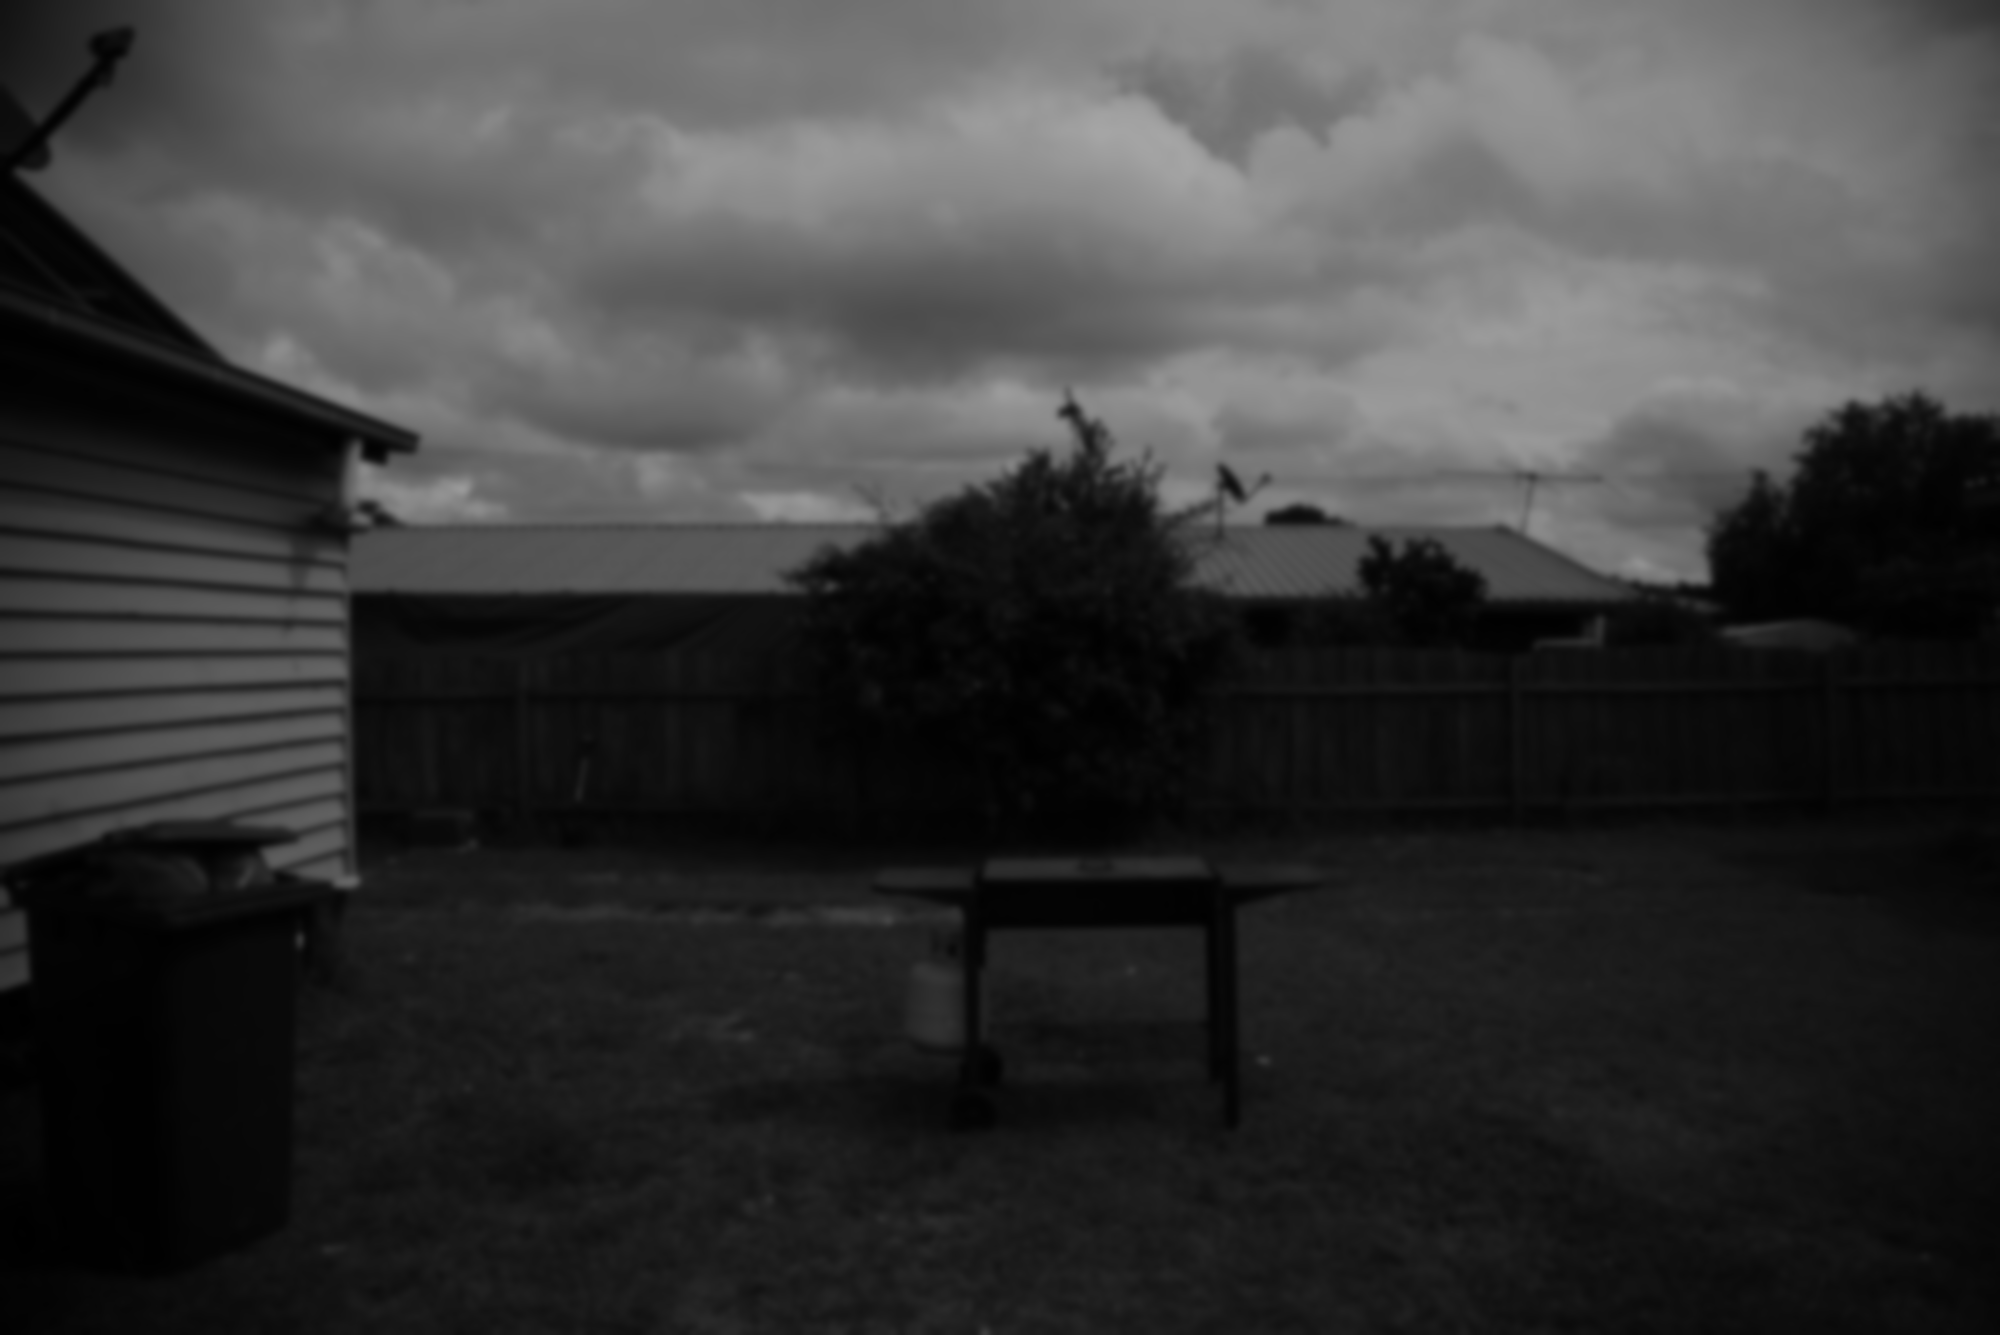
\includegraphics[trim={20cm 25cm 25cm 10cm},clip,width=\textwidth]{Generated/Garden_gaussian21filter.png}
		\caption{Gaussian filter (kernel 21) on Garden (cropped)}
		\label{fig:gaussian21_Garden}
	\end{subfigure}
	\hfill
	\begin{subfigure}{0.3\textwidth}
		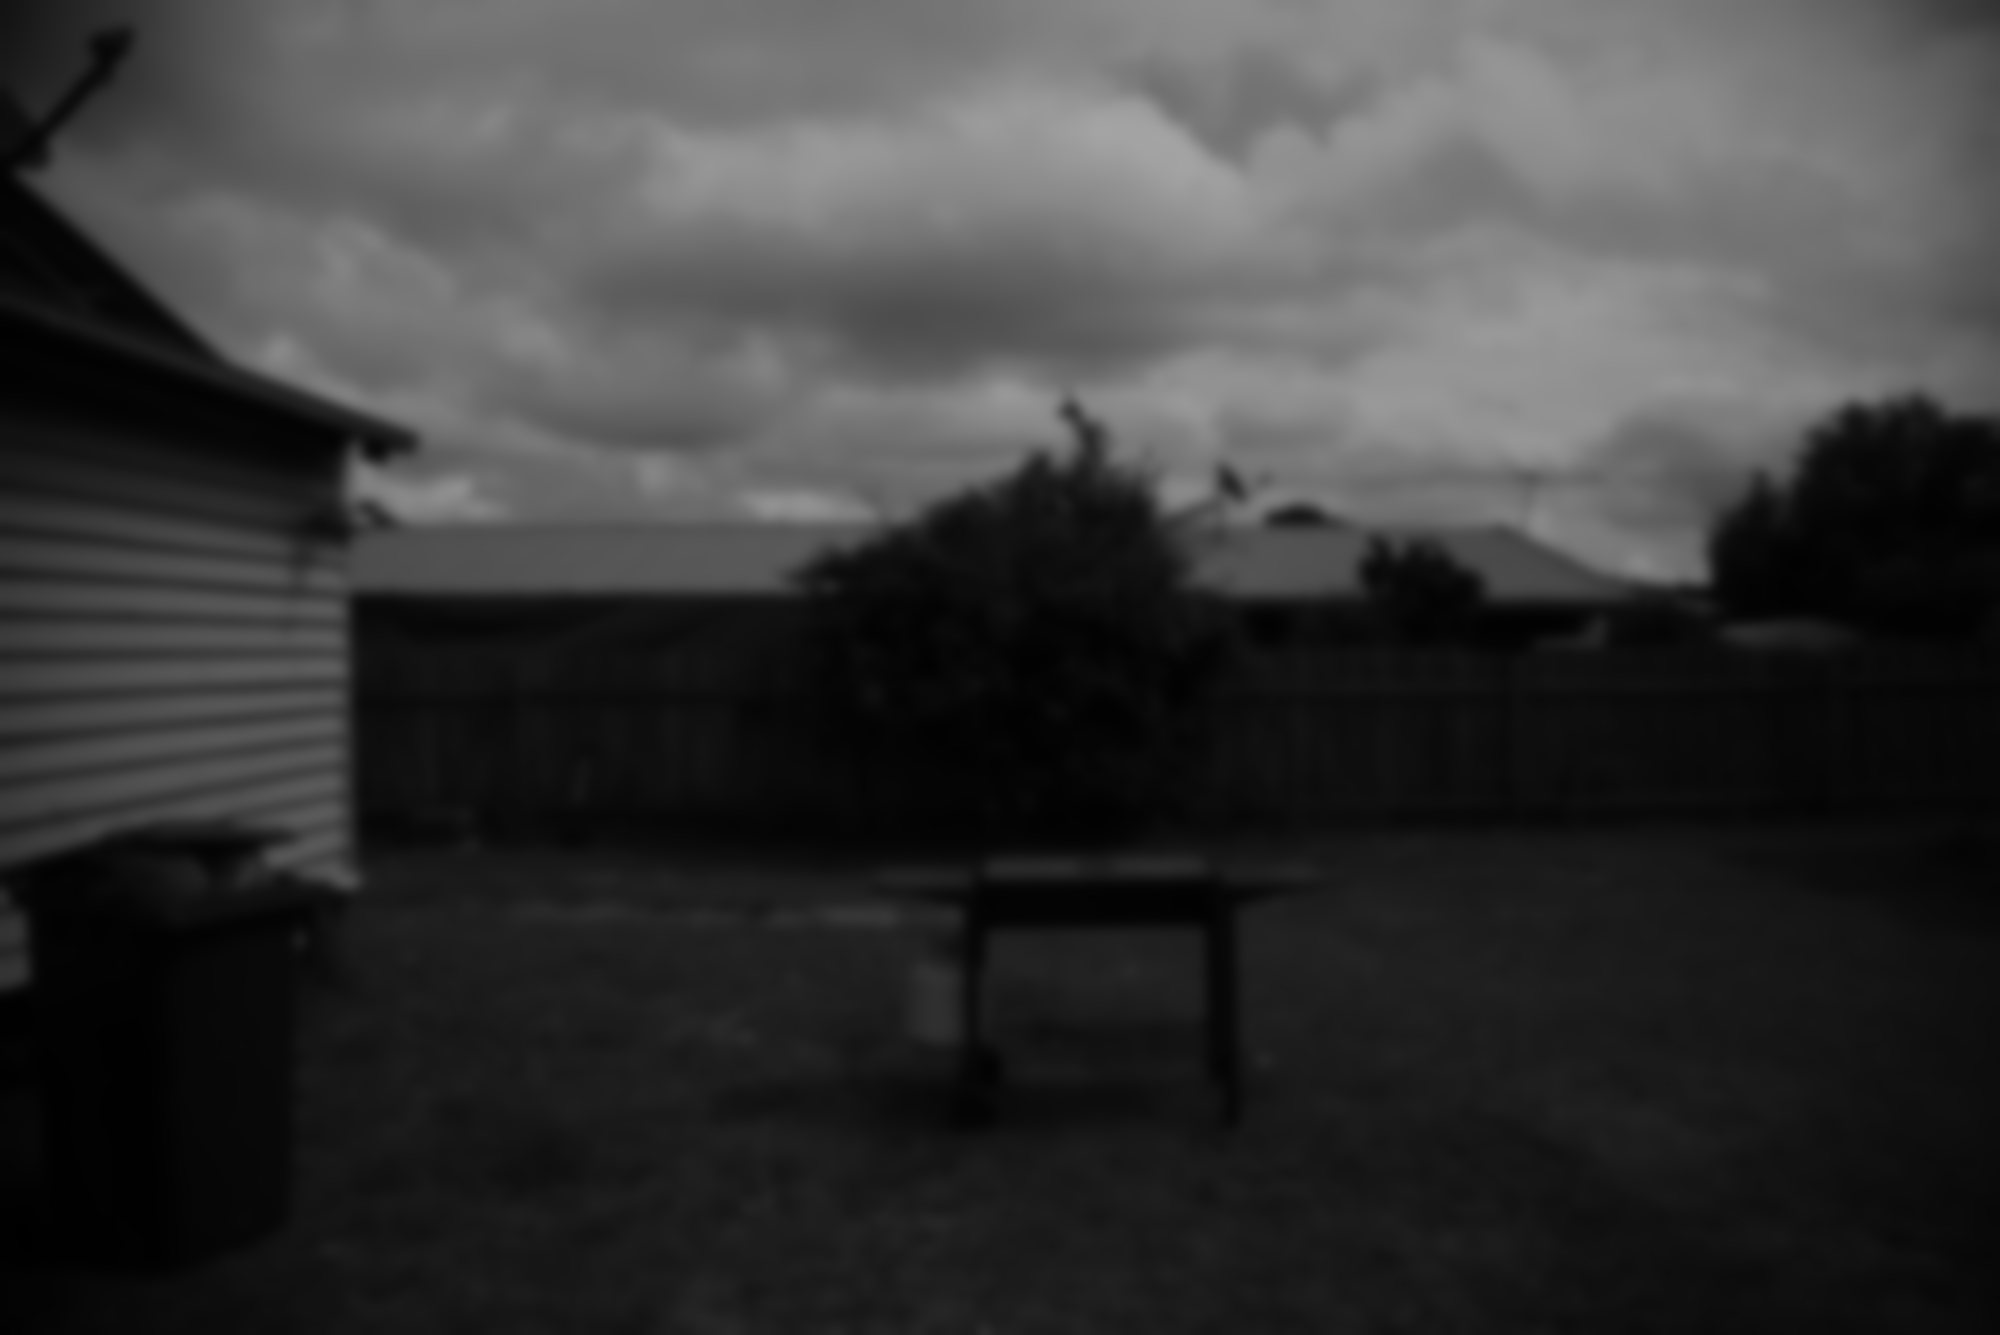
\includegraphics[trim={20cm 25cm 25cm 10cm},clip,width=\textwidth]{Generated/Garden_gaussian41filter.png}
		\caption{Gaussian filter (kernel 41) on Garden (cropped)}
		\label{fig:gaussian41_Garden}
	\end{subfigure}
	\caption{Gaussian filter}
\end{figure}


\section*{Task 5}
Histograms are generated from grayscale images (1 channel) using \texttt{cv::calcHist}.
Histograms change based on the number of bins used ($[0, 255]$ for \texttt{uchar} images, for each channel): histograms with 255 bins represent the frequency for each single gray-level (Figures \labelcref{fig:hist255_Lena,fig:hist255_Astronaut,fig:hist255_Garden}); using less bins (10 in the example) levels are grouped together (in the example groups of 255/10) (Figures \labelcref{fig:hist10_Lena,fig:hist10_Astronaut,fig:hist10_Garden}).
\begin{figure}[H]
	\centering
	\begin{subfigure}{0.4\textwidth}
		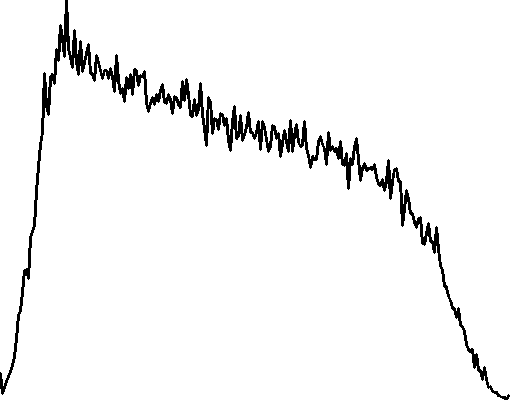
\includegraphics[width=\textwidth]{Generated/Lena_corrupted_histogramOneChannel255bins.png}
		\caption{Histogram with 255 bins, corrupted Lena}
		\label{fig:hist255_Lena}
	\end{subfigure}
	\hfill
	\begin{subfigure}{0.4\textwidth}
		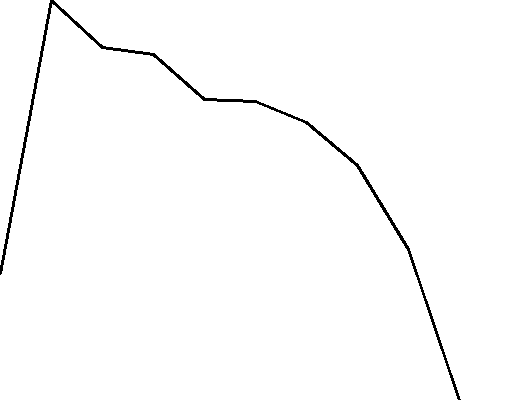
\includegraphics[width=\textwidth]{Generated/Lena_corrupted_histogramOneChannel10bins.png}
		\caption{Histogram with 10 bins, corrupted Lena}
		\label{fig:hist10_Lena}
	\end{subfigure}

	\begin{subfigure}{0.4\textwidth}
		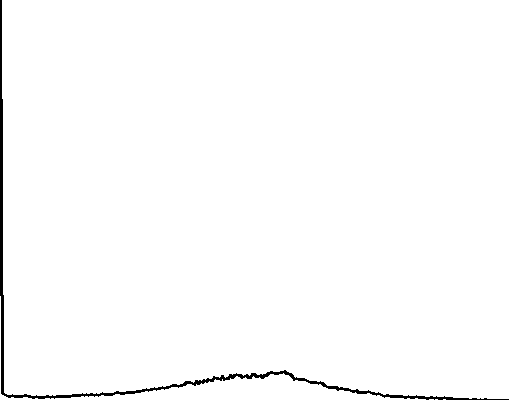
\includegraphics[width=\textwidth]{Generated/Astronaut_salt_pepper_histogramOneChannel255bins.png}
		\caption{Histogram with 255 bins, corrupted Astronaut}
		\label{fig:hist255_Astronaut}
	\end{subfigure}
	\hfill
	\begin{subfigure}{0.4\textwidth}
		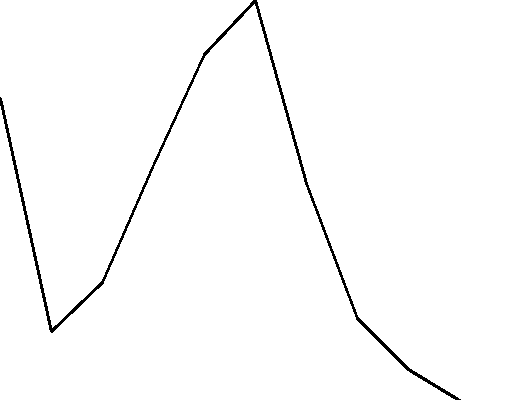
\includegraphics[width=\textwidth]{Generated/Astronaut_salt_pepper_histogramOneChannel10bins.png}
		\caption{Histogram with 255 bins, corrupted Astronaut}
		\label{fig:hist10_Astronaut}
	\end{subfigure}

	\begin{subfigure}{0.4\textwidth}
		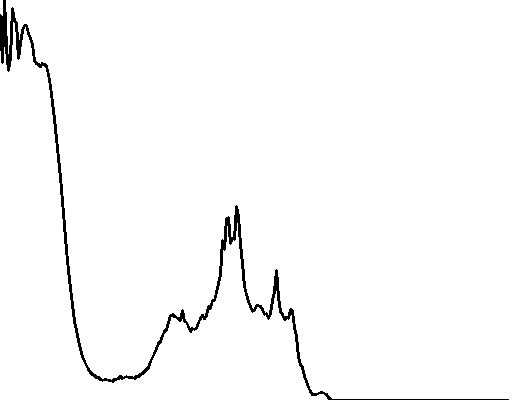
\includegraphics[width=\textwidth]{Generated/Garden_histogramOneChannel255bins.png}
		\caption{Histogram with 255 bins, Garden}
		\label{fig:hist255_Garden}
	\end{subfigure}
	\hfill
	\begin{subfigure}{0.4\textwidth}
		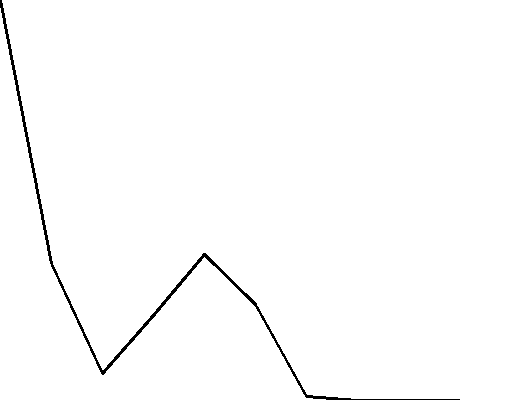
\includegraphics[width=\textwidth]{Generated/Garden_histogramOneChannel10bins.png}
		\caption{Histogram with 255 bins, Garden}
		\label{fig:hist10_Garden}
	\end{subfigure}
	\caption{Histograms}
	\label{fig:histograms}
\end{figure}


\section*{Task 6}
Histogram equalization is applied using \texttt{cv::equalizeHist}.
Results are shown in figure \ref{fig:eqHist}.
\begin{figure}[H]
	\centering
	\begin{subfigure}{0.3\textwidth}
		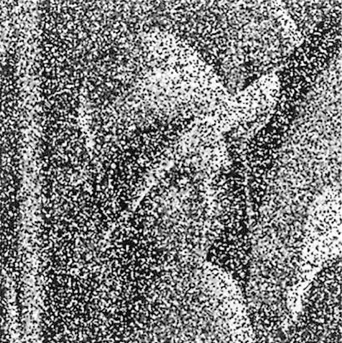
\includegraphics[width=\textwidth]{Generated/Lena_corrupted_eqHistOneChannel255bins.png}
		\caption{Histogram equalization (255 bins), corrupted Lena}
	\end{subfigure}
	\hfill
	\begin{subfigure}{0.3\textwidth}
		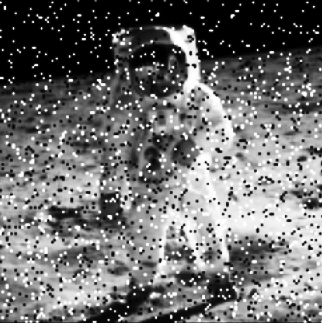
\includegraphics[width=\textwidth]{Generated/Astronaut_salt_pepper_eqHistOneChannel255bins.png}
		\caption{Histogram equalization (255 bins), corrupted Astronaut}
	\end{subfigure}
	\hfill
	\begin{subfigure}{0.3\textwidth}
		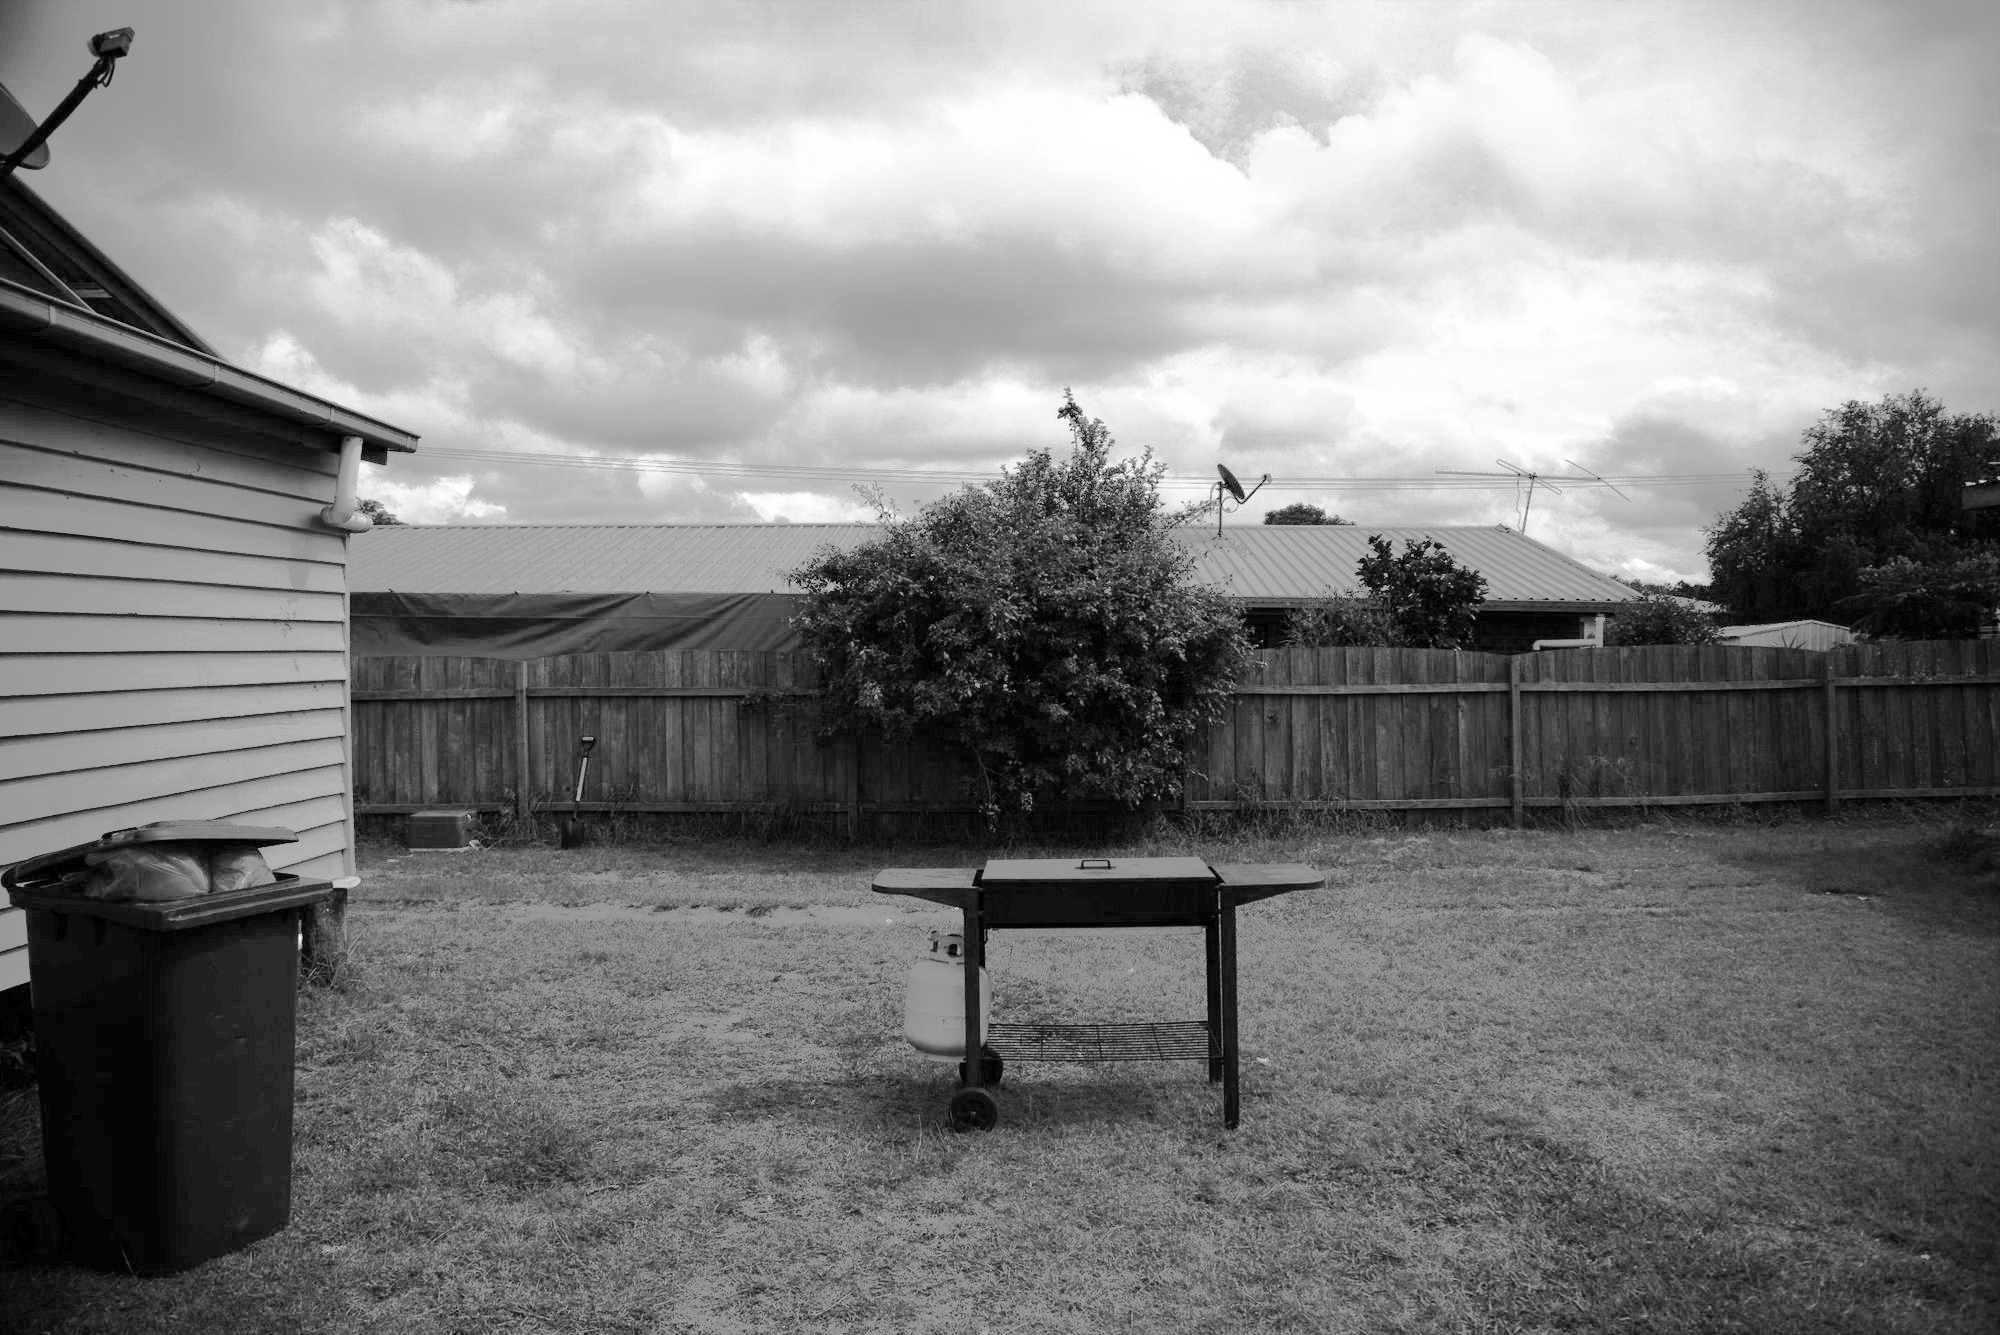
\includegraphics[width=\textwidth]{Generated/Garden_eqHistOneChannel255bins.png}
		\caption{Histogram equalization (255 bins), Garden}
	\end{subfigure}
	\caption{Histogram equalization applied on images}
	\label{fig:eqHist}
\end{figure}


\end{document}